\documentclass[16pt, a4paper]{article}
% \usepackage[utf8]{inputenc}
\usepackage{graphicx}
\usepackage{geometry}
\usepackage{amsmath}
\usepackage{cleveref}
\geometry{a4paper, margin=0.5in}
\usepackage[font=small,labelfont=bf]{caption}

\newcommand{\beginsupplement}{%
        \setcounter{figure}{0}
        \renewcommand{\thefigure}{\arabic{figure}}%
        \renewcommand{\figurename}{Appendix 2 figure}
     }
     
\newcommand{\beginmain}{%
    \setcounter{figure}{0}
    \renewcommand{\thefigure}{\arabic{figure}}%
     }
     
\newcommand{\begingraphical}{%
    \setcounter{figure}{0}
    \renewcommand{\thefigure}{G\arabic{figure}}%
     }

\begin{document}
\pagenumbering{gobble}

\begingraphical 
\begin{figure}[ht!]
    \centering
    \includegraphics[width = 0.75\paperwidth, height=0.6\paperheight, keepaspectratio]{Supplementary_Figures/FigG01.pdf}
    \caption{Graphical Abstract}
    \label{Fig G1}
\end{figure}

\clearpage

\beginmain
\begin{figure}[ht!]
        \centering
        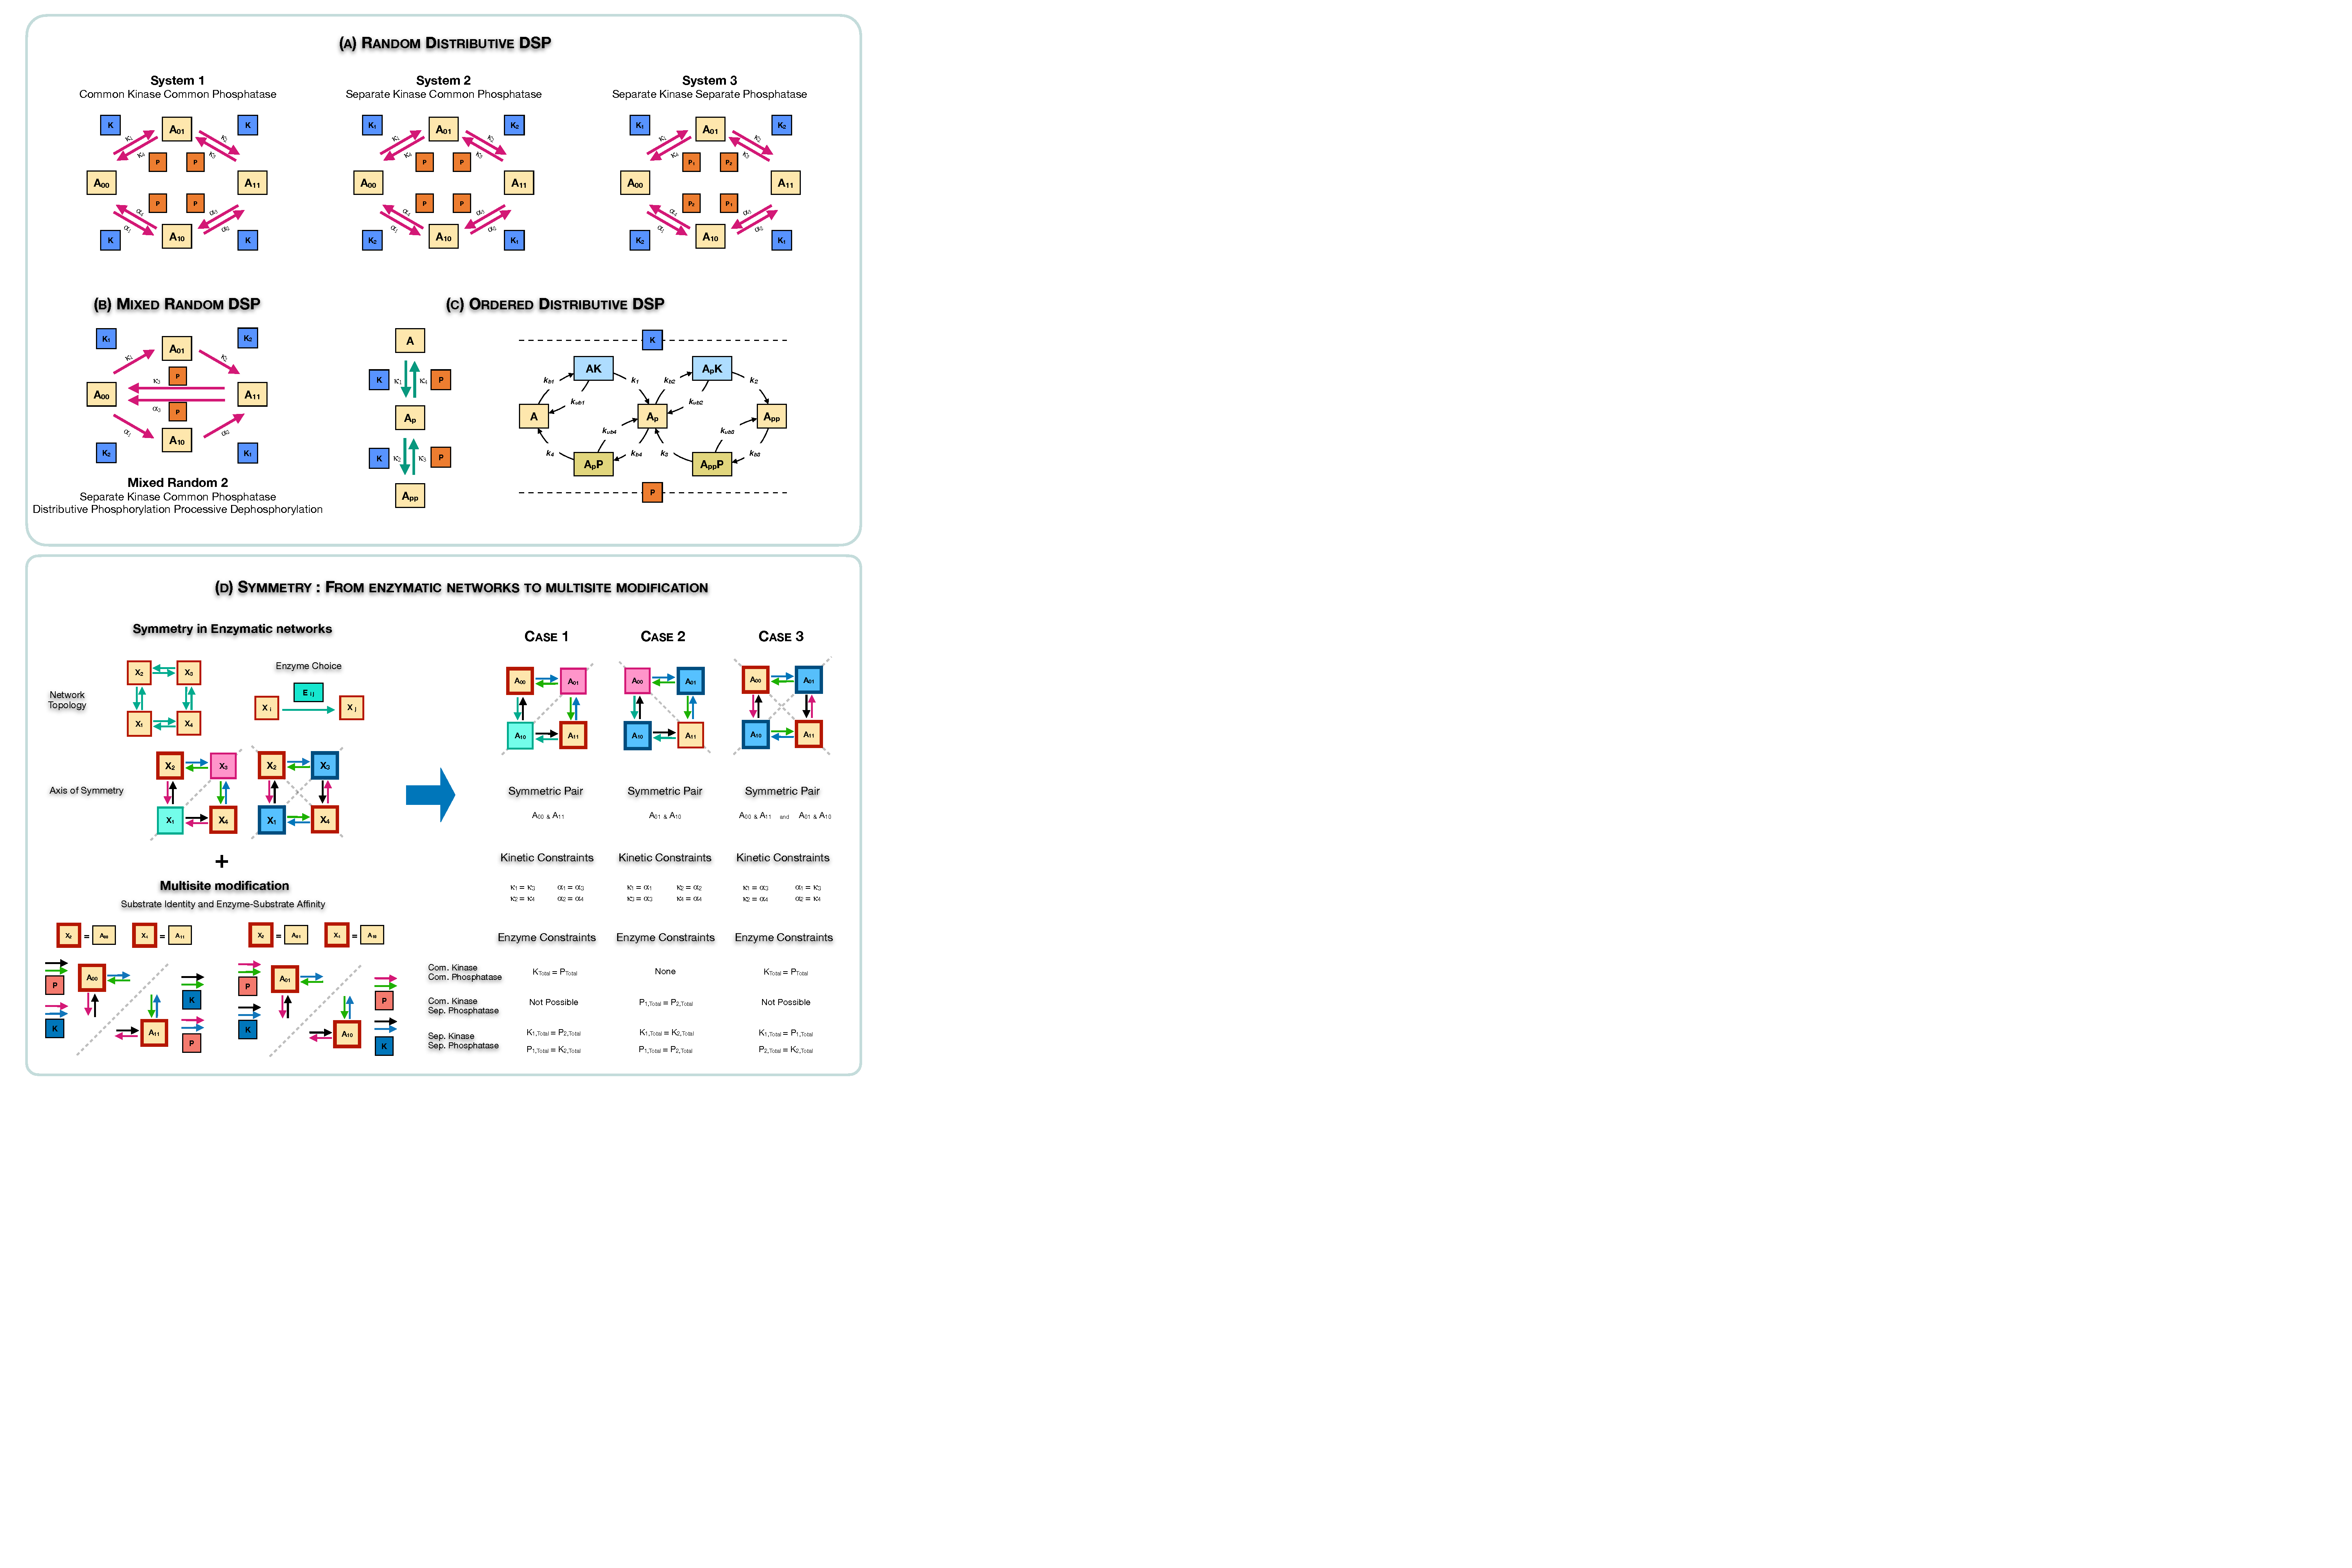
\includegraphics[width = 0.9\paperwidth, height = 0.6\paperheight, keepaspectratio]{Supplementary_Figures/Fig01.pdf}
        \caption{(A-C). \textbf{Schematic representation of the various multisite phosphorylation networks considered in the paper.} (A) depicts the core networks while (B,C) serve as suitable contrasts to illustrate basic points. The labels $\kappa_i$, $\alpha_i$ in the schematic represent the triplet of binding, unbinding and catalytic rate constants involved in the enzyme modification for the $i^{th}$ modification (on each leg of the network). Detailed model description is provided in Appendix 2 - \Cref{Fig S10}. (A) shows the various random (distributive) double site phosphorylation (DSP) networks (the focal point of the study) with different combinations of enzyme action (common kinase and common phosphatase, separate kinase and common phosphatase, and separate kinase and separate phosphatase). (B) shows the random DSP with distributive phosphorylation and processive dephosphorylation (depicted for simplicity as direct arrows from $A_{11} \rightarrow A_{00}$) with separate kinase and common phosphatase (Model: Mixed Random 2). (C) shows the ordered distributive DSP with common kinase and common phosphatase, and an expanded description of reaction mechanism showing in detail the binding, unbinding and catalytic action for each modification step. (D). \textbf{Schematic representation of the three different classes of symmetries in the random DSP networks considered in this study.} 
        The different symmetries are depicted in the right hand panel. In each case, the axis of symmetry is depicted, and nodes of the network on either side of this axis (enclosed in a boundary of the same colour) have equal concentration. Identically coloured arrows in schematics are indicative of equal kinetic rate constants (for the corresponding triplet of binding/unbinding/catalysis) and equal total concentrations of enzymes involved. The associated kinetic and enzymatic requirements required for enforcing symmetries are also listed. These are key ingredients in establishing symmetry in the reaction network. 
        The origins of these symmetries can be conceptualized and visualized by examining an enzymatic network with a ``square" topology (left hand panel), where every reaction is mediated by an enzyme. Such networks can have symmetry about one axis or two axes.
        Now examining the single axis reflection symmetry in multi-site modification results in two possibilities of symmetric nodes (the pair ($A_{00},A_{11}$) and ($A_{01},A_{10}$)). In each case - symmetry requires different pairs of reactions (depicted by identically coloured arrows) to have equivalent rates and enzyme amounts. Importantly, in the $A_{11} = A_{00}$ case these pairs of reactions are associated with enzymes of different kinds, while in the $A_{01}=A_{10}$ case they are associated with enzymes of the same kind. While this is depicted for a single kinase and a single phosphatase it applies to any combination of common/separate kinase and phosphatase. This dichotomy underscores the difference between case 1 and case 2 symmetry. 
        Overall this conceptualization allows us to obtain the three symmetries along with the kinetic and enzymatic requirements shown in the right hand panel.}
        \label{Fig 1}
\end{figure}

\clearpage
\begin{figure}[h!]
    \centering
    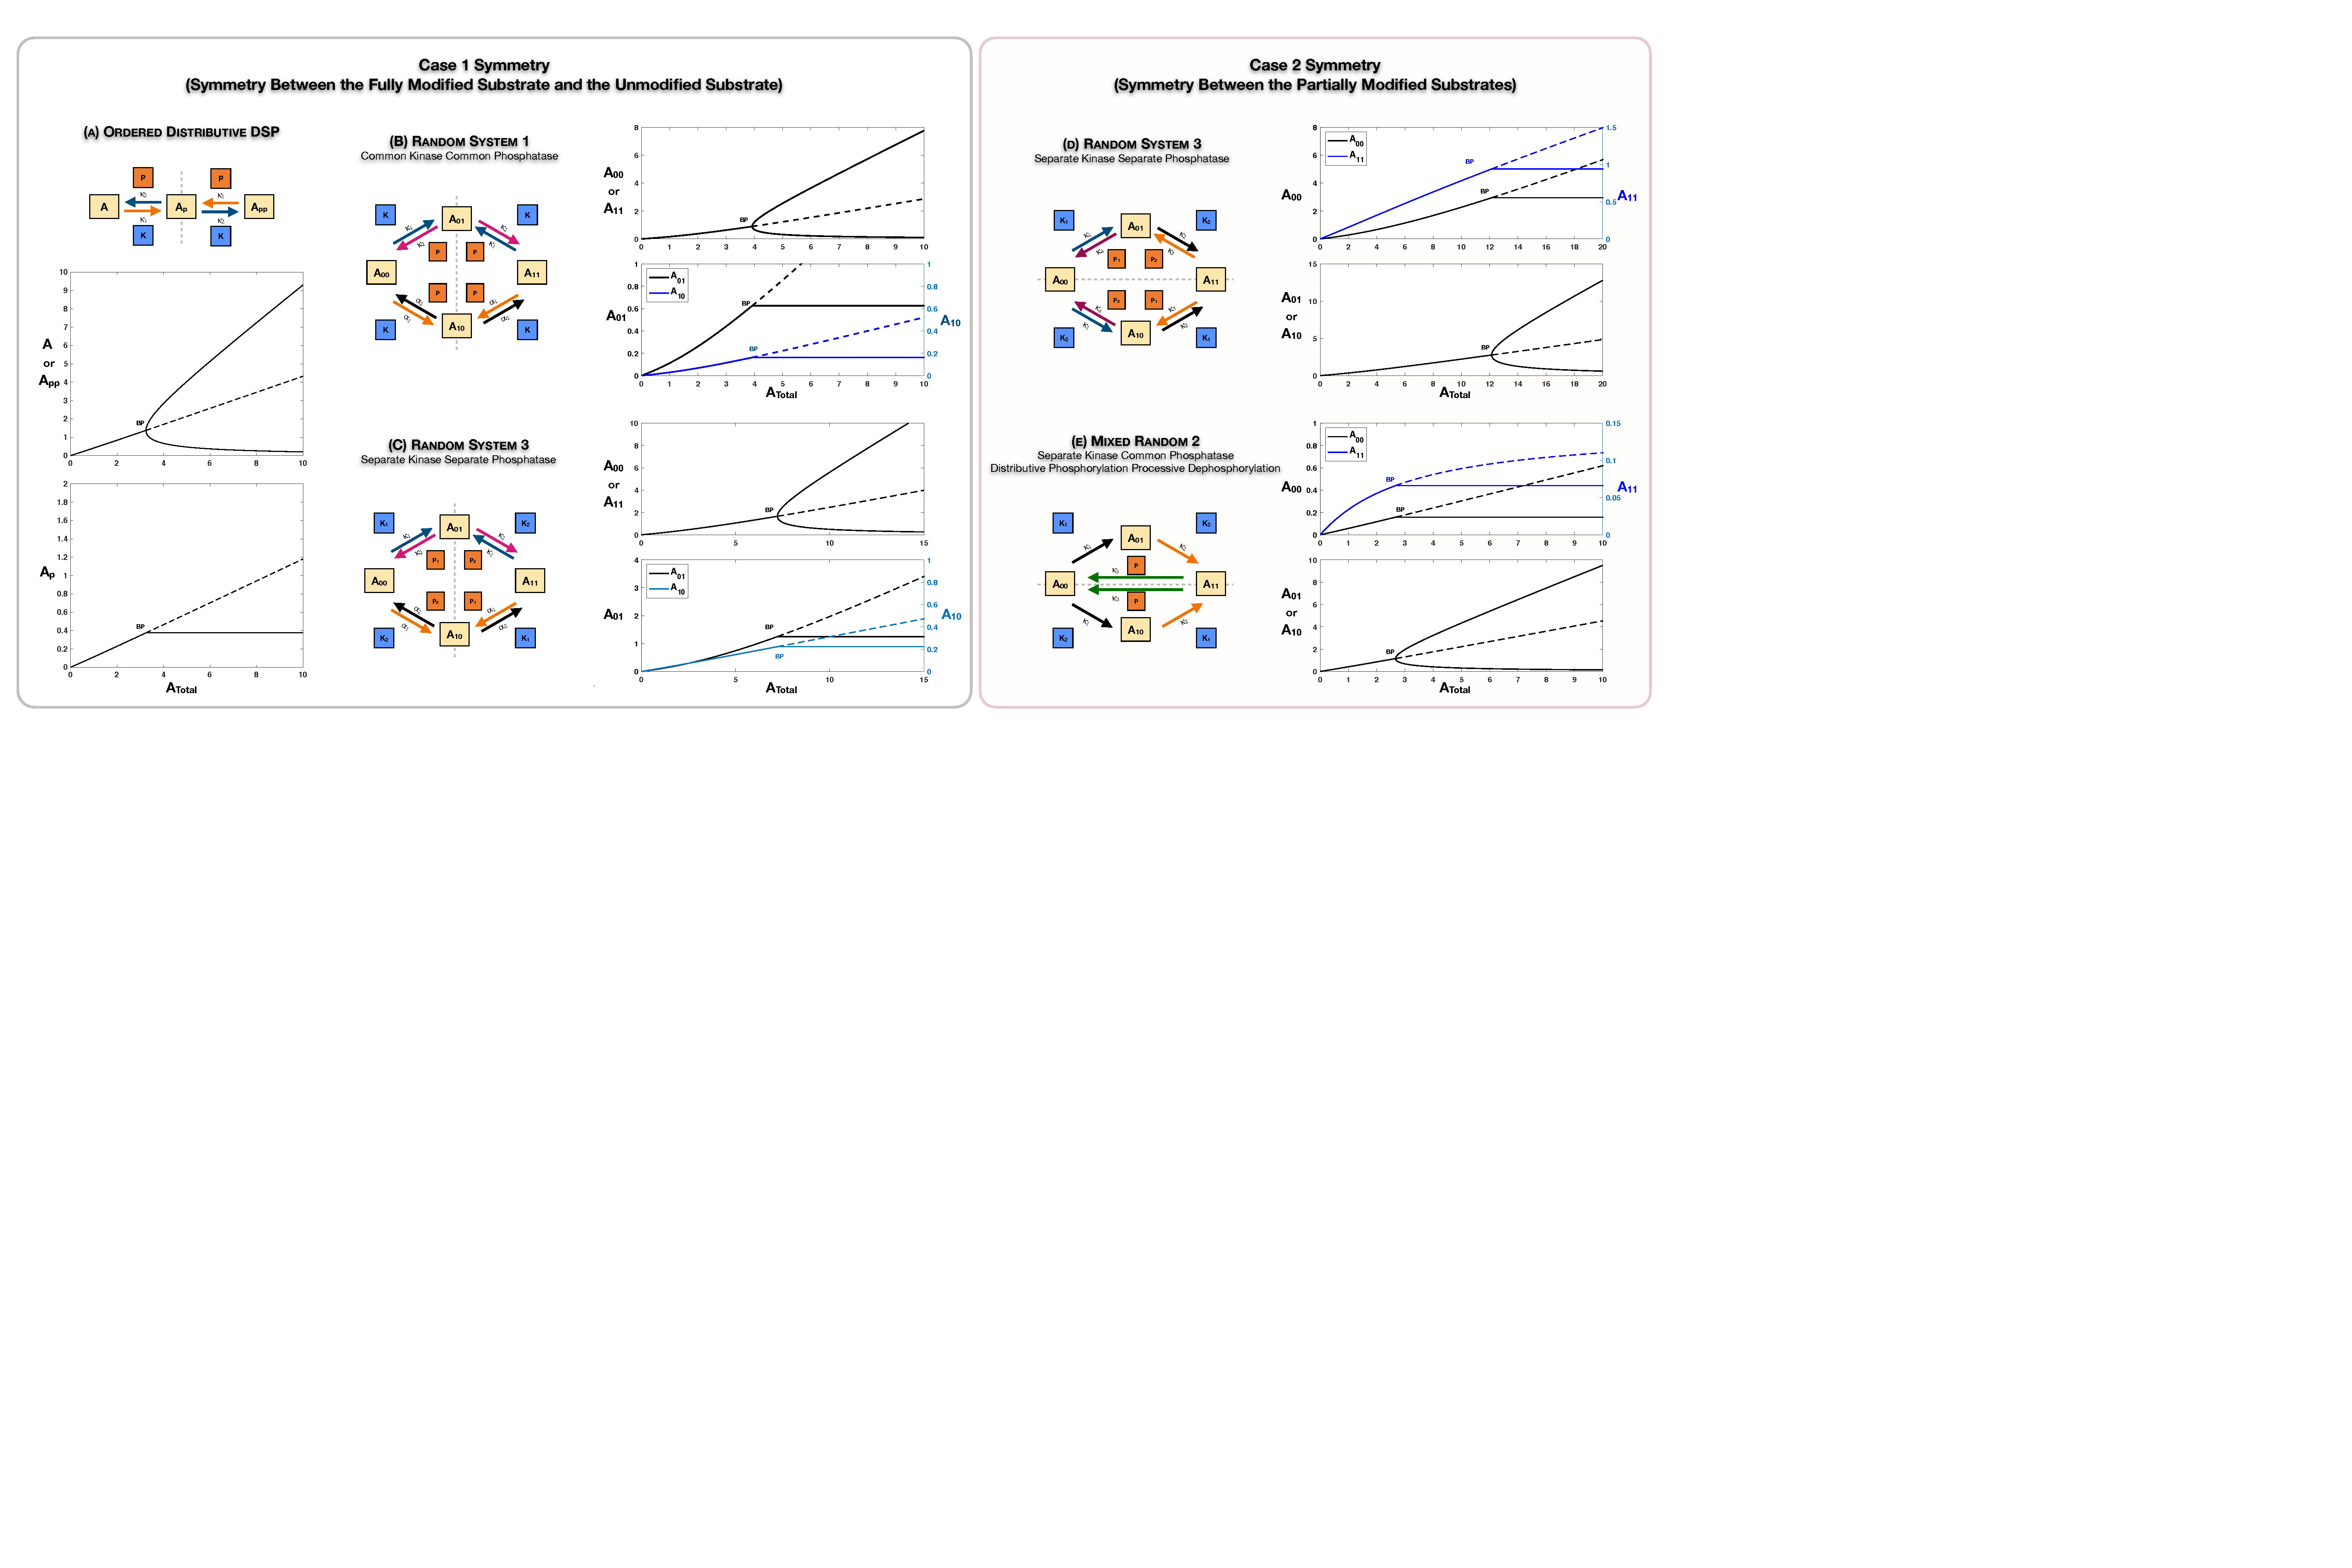
\includegraphics[angle = 0, width = 0.85\paperwidth, keepaspectratio]{Supplementary_Figures/Fig02.pdf}
    \caption{\textbf{Case 1 and case 2 symmetry breaking in various double site phosphorylation networks.}
    (A-C). Case 1 symmetry breaking in distributive  DSP: (A), ordered DSP with common kinase and common phosphatase, (B), random DSP with common kinase and common phosphatase, (C), random  DSP with separate kinase and separate phosphatase. Note that in these cases the concentrations of the partially modified substrates are fixed after symmetry breaking  (in the symmetry broken state) in the bifurcation diagrams.
    (D-E). Case 2 symmetry breaking: (D), random  DSP with separate kinase and separate phosphatase,  (E), mixed random DSP with distributive phosphorylation through separate kinases and processive dephosphorylation through common phosphatase. Note that in these cases the concentrations of the fully modified and unmodified substrate are fixed after symmetry breaking (in the symmetry-broken state) in the bifurcation diagrams.
    [Dashed lines indicate unstable steady states, while solid lines represent stable steady states in the bifurcation diagram. Dashed lines in the  schematic represent axis of symmetry of the network. BP: Pitchfork bifurcation]}
    \label{Fig 2}
\end{figure}

\clearpage
\begin{figure}[h!]
    \centering
    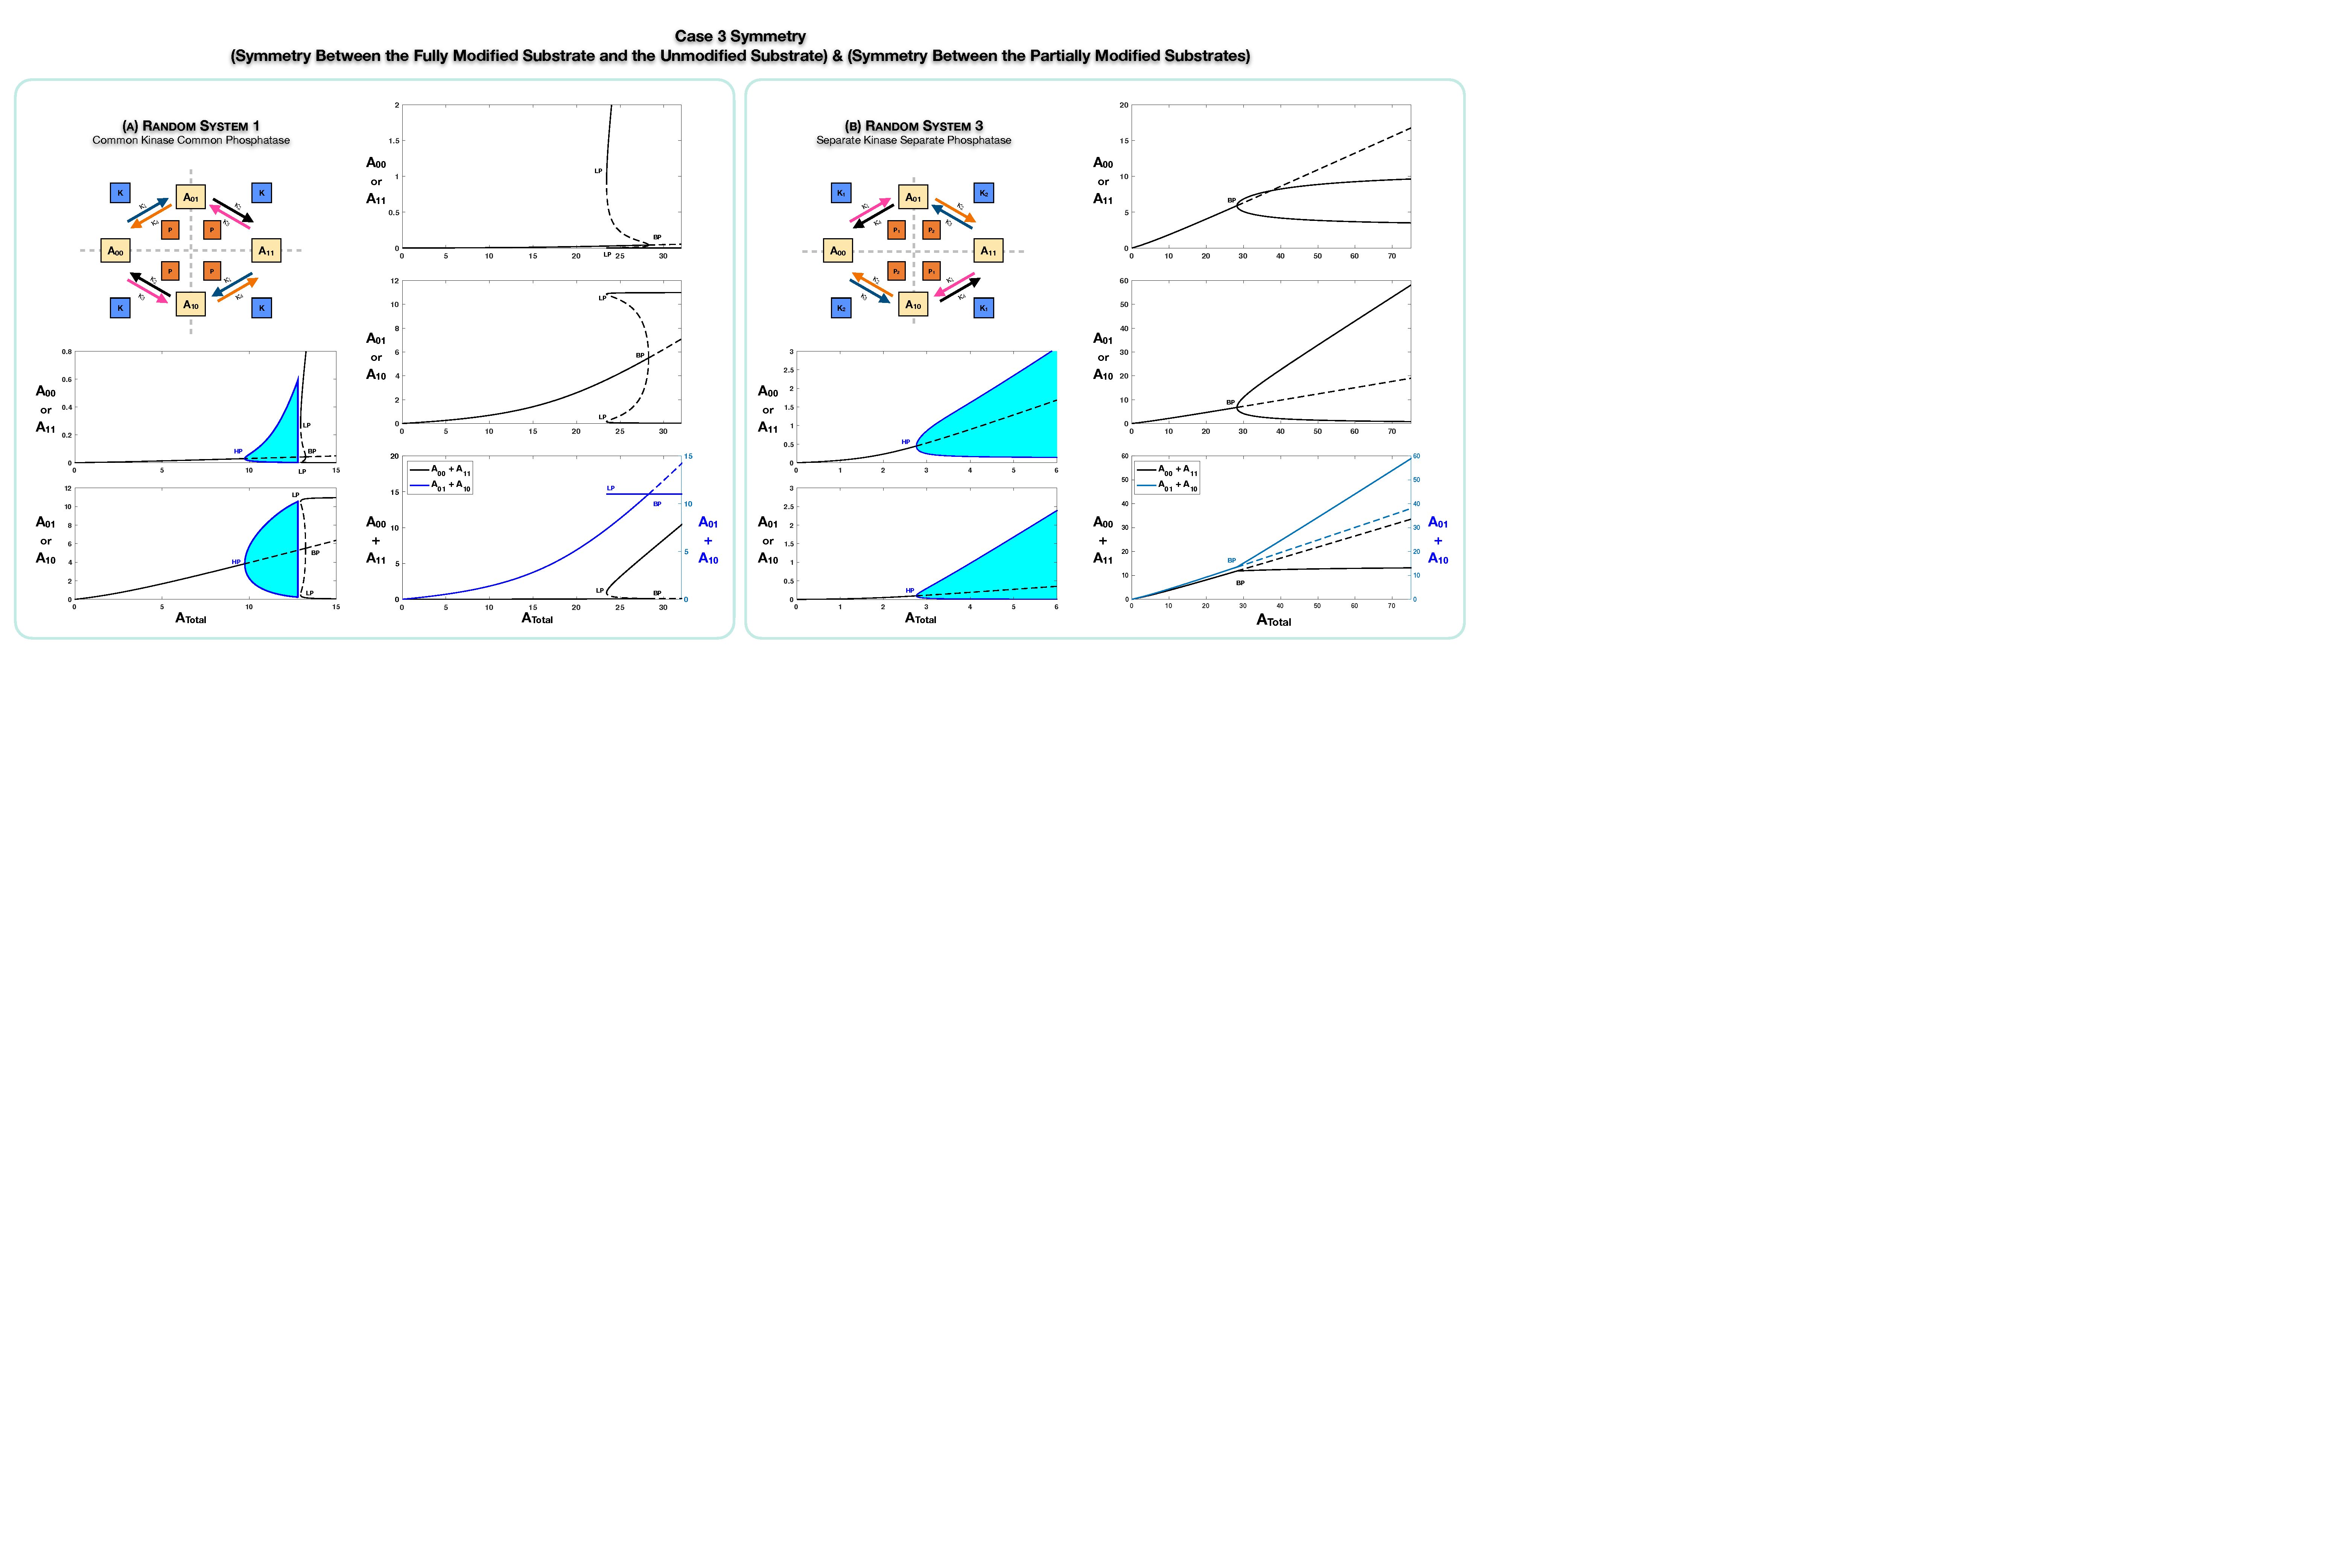
\includegraphics[angle = 0, width = 0.85\paperwidth, keepaspectratio]{Supplementary_Figures/Fig03.pdf}
    \caption{\textbf{Case 3 symmetry breaking in various double site phosphorylation networks.}
    (A) shows case 3 symmetry breaking in random DSP with common kinase and common phosphatase. The symmetric steady state is capable of losing stability either through a Hopf bifurcation leading to oscillations, which is followed by symmetry breaking through a subcritical Pitchfork bifurcation eventually leading to stable asymmetric steady states (Column 1), or just by breaking symmetry leading to asymmetric branches through a subcritical Pitchfork bifurcation which eventually becomes stable (Column 2). As seen in the plots, both symmetries simultaneously break. Note that the sum of the concentrations of the partially modified substrates is fixed in the asymmetric states in the bifurcation diagrams.
    Symmetry-breaking via a supercritical pitchfork bifurcation, as seen previously in other cases, can also be seen (Appendix 2 - \Cref{Fig S2}).
    (B) shows case 3 symmetry breaking in random DSP with separate kinase and separate phosphatase. The symmetric steady state is capable of losing stability either through a Hopf bifurcation leading to oscillations (Column 1), or by breaking symmetry leading to two stable asymmetric branches through a supercritical Pitchfork bifurcation (Column 2). Note that the sum of the concentrations of the completely modified and completely unmodified substrates is approximately constant in the asymmetric steady states in the bifurcation diagram. (However case 3 symmetry breaking in this network is also capable of providing approximate concentration robustness in the sum of the concentrations of partial substrate forms - see main text and Appendix 2 - \Cref{Fig S4}).
    [Dotted lines indicate unstable steady states, while solid lines represent stable steady states in the bifurcation diagram. Shaded regions in the bifurcation diagram indicate regions of oscillations and the blue lines indicate bounds on concentrations during such oscillations. BP: Pitchfork bifurcation, HP: Hopf bifurcation, LP: Saddle node bifurcation.]}
    \label{Fig 3}
\end{figure}

\clearpage
\begin{figure}[h!]
    \centering
    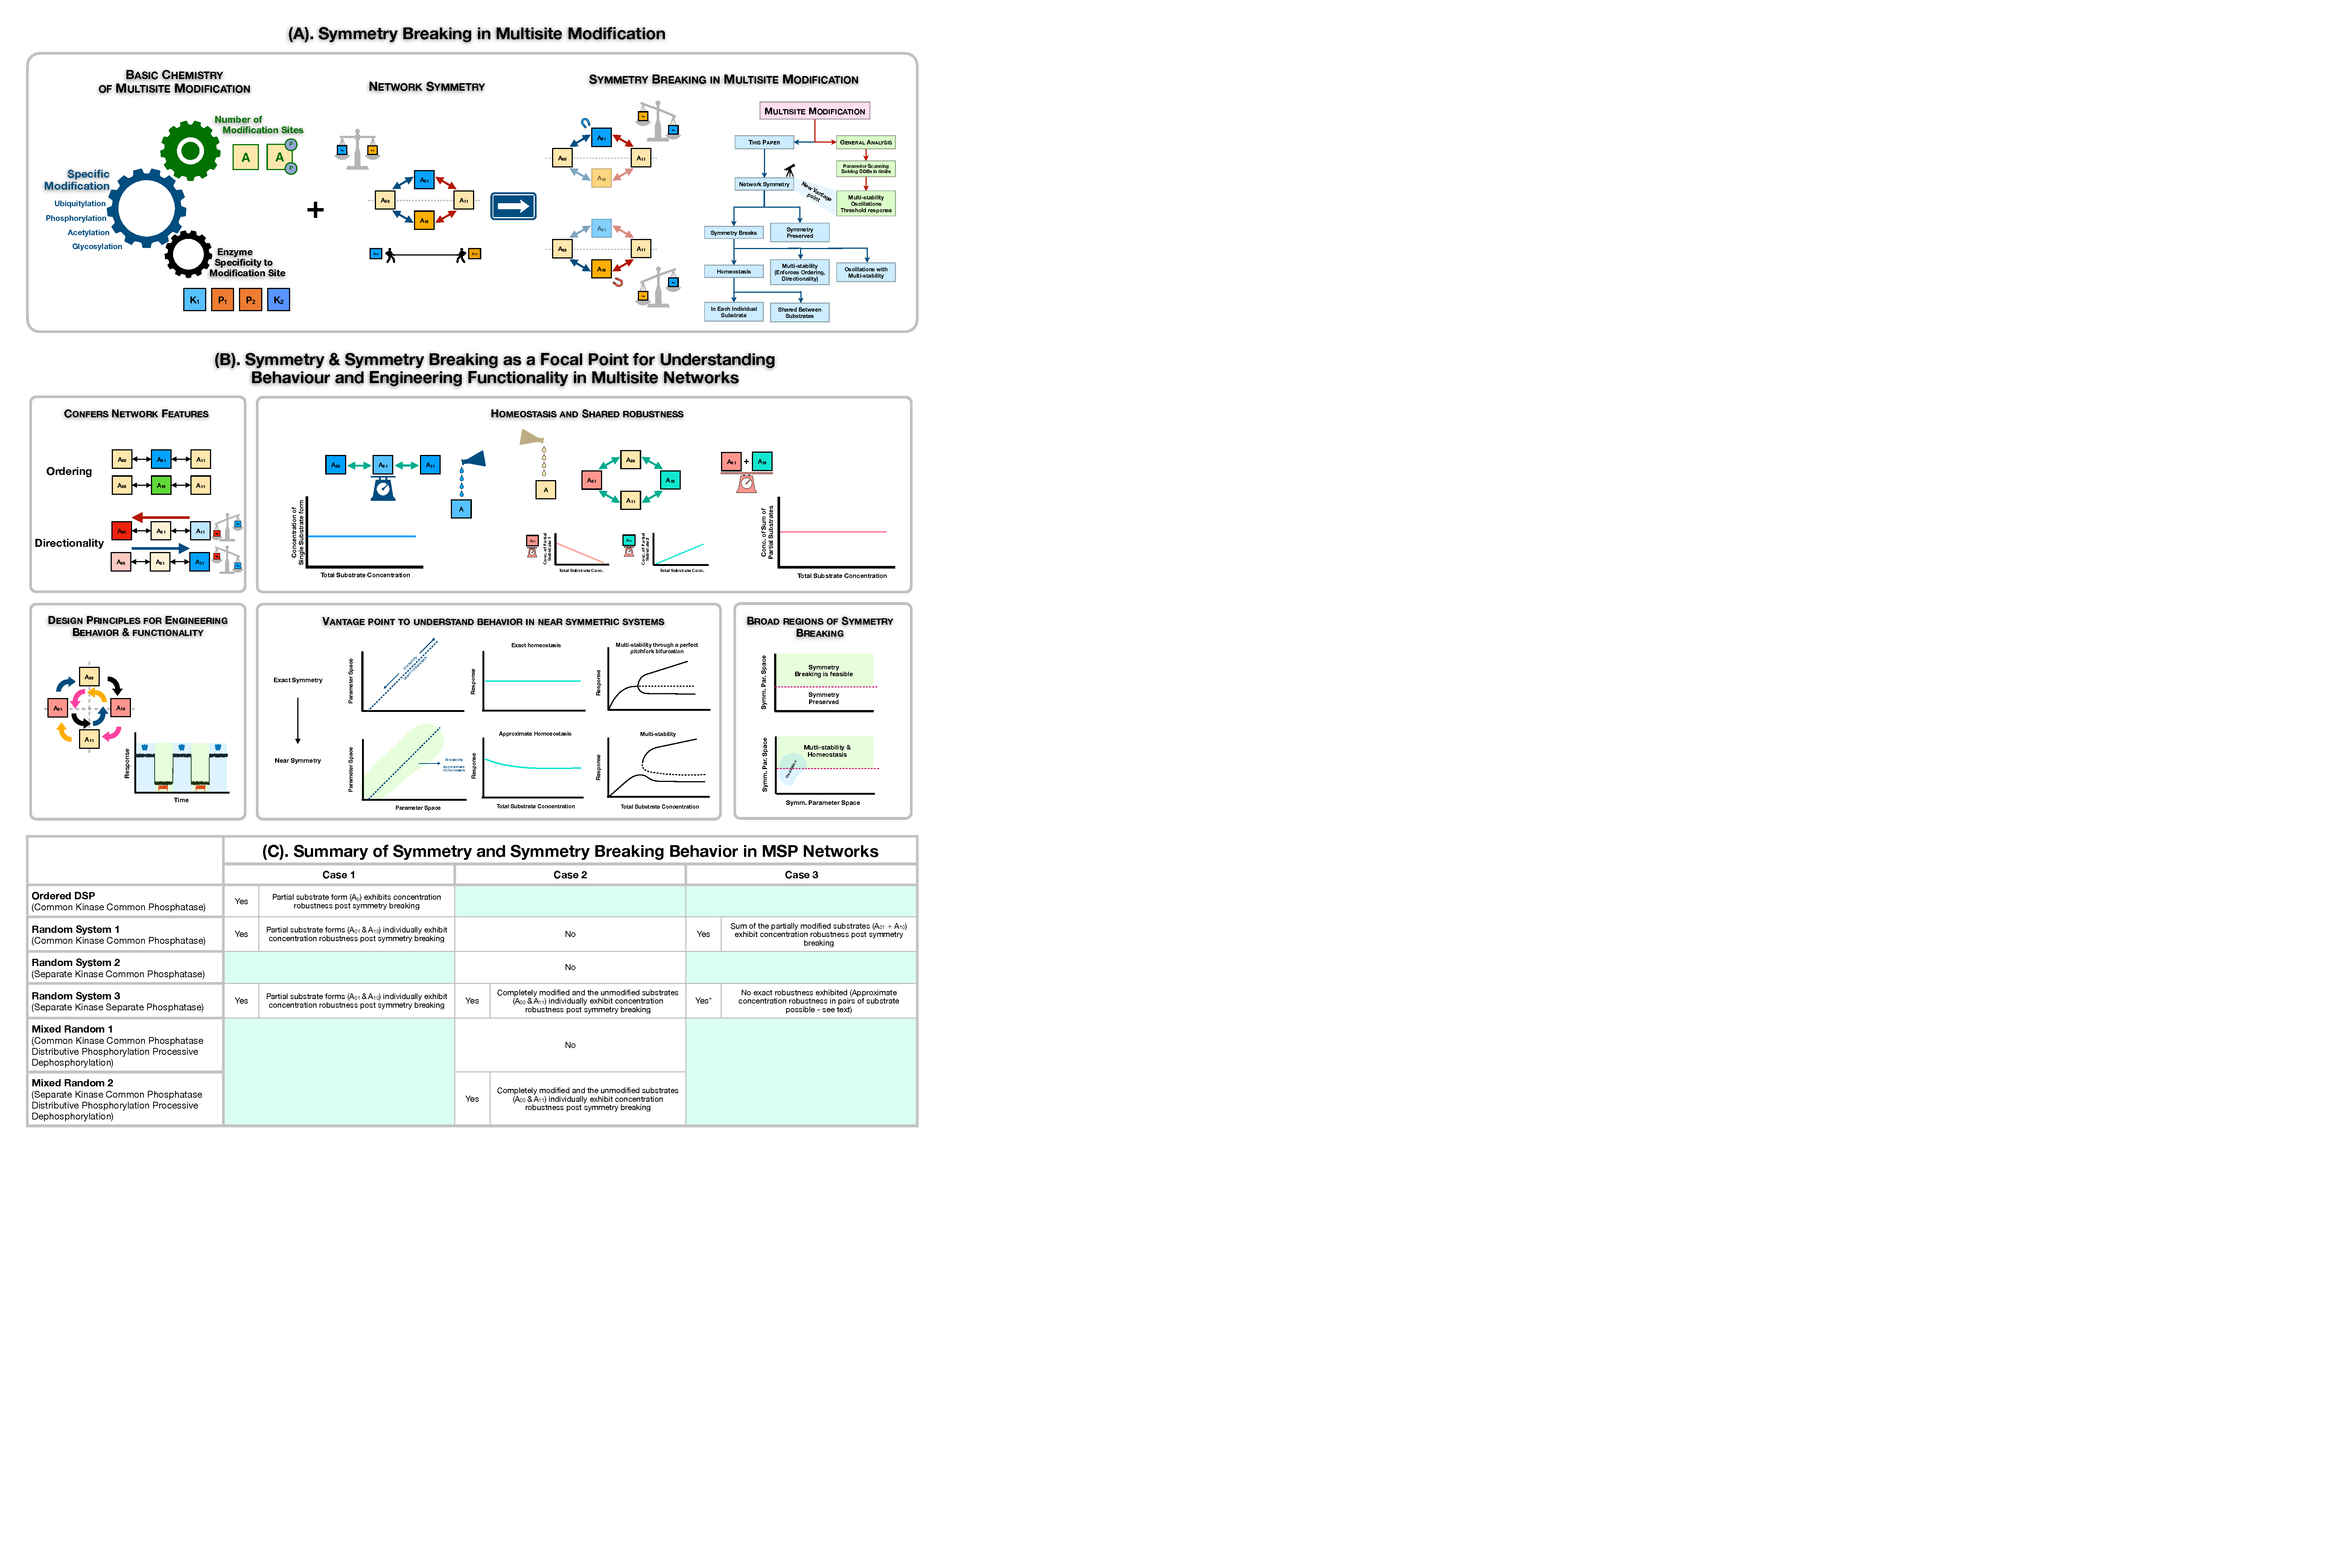
\includegraphics[angle = 0, height = \paperwidth, width = \paperwidth, keepaspectratio]{Supplementary_Figures/Fig04.pdf}
    \caption{A. Schematic representation of realization of symmetry and symmetry breaking in multisite modification networks through the interplay of basic biochemistry of post translational protein modification and network symmetry. The analysis of the multisite network through symmetry and symmetry breaking reveals the underpinnings of new network features, and serves as a rich and distinct vantage point to understand information processing behavior in multisite modification networks. B. Symmetry breaking as a new vista for understanding behavior and engineering functionality in multi-site modification networks: Symmetry breaking can confer network features such as ordering and directionality to MSP networks, limit the range of oscillations and enable robust homeostasis for individual or combinations of substrates.
    %It can help realise various robust information processing characteristics in MSP networks such as homeostasis in a single substrate and in a combination of substrates. 
    It also provides key insights on the origin of behaviors in networks which are not far from symmetry. C. A tabular summary of the presence and absence of symmetry and symmetry breaking in MSP networks, along with features of the symmetry broken states (exact absolute concentration robustness).}
    \label{Fig 4}
\end{figure}

\clearpage
\beginsupplement

\begin{figure}[ht!]
    \centering
    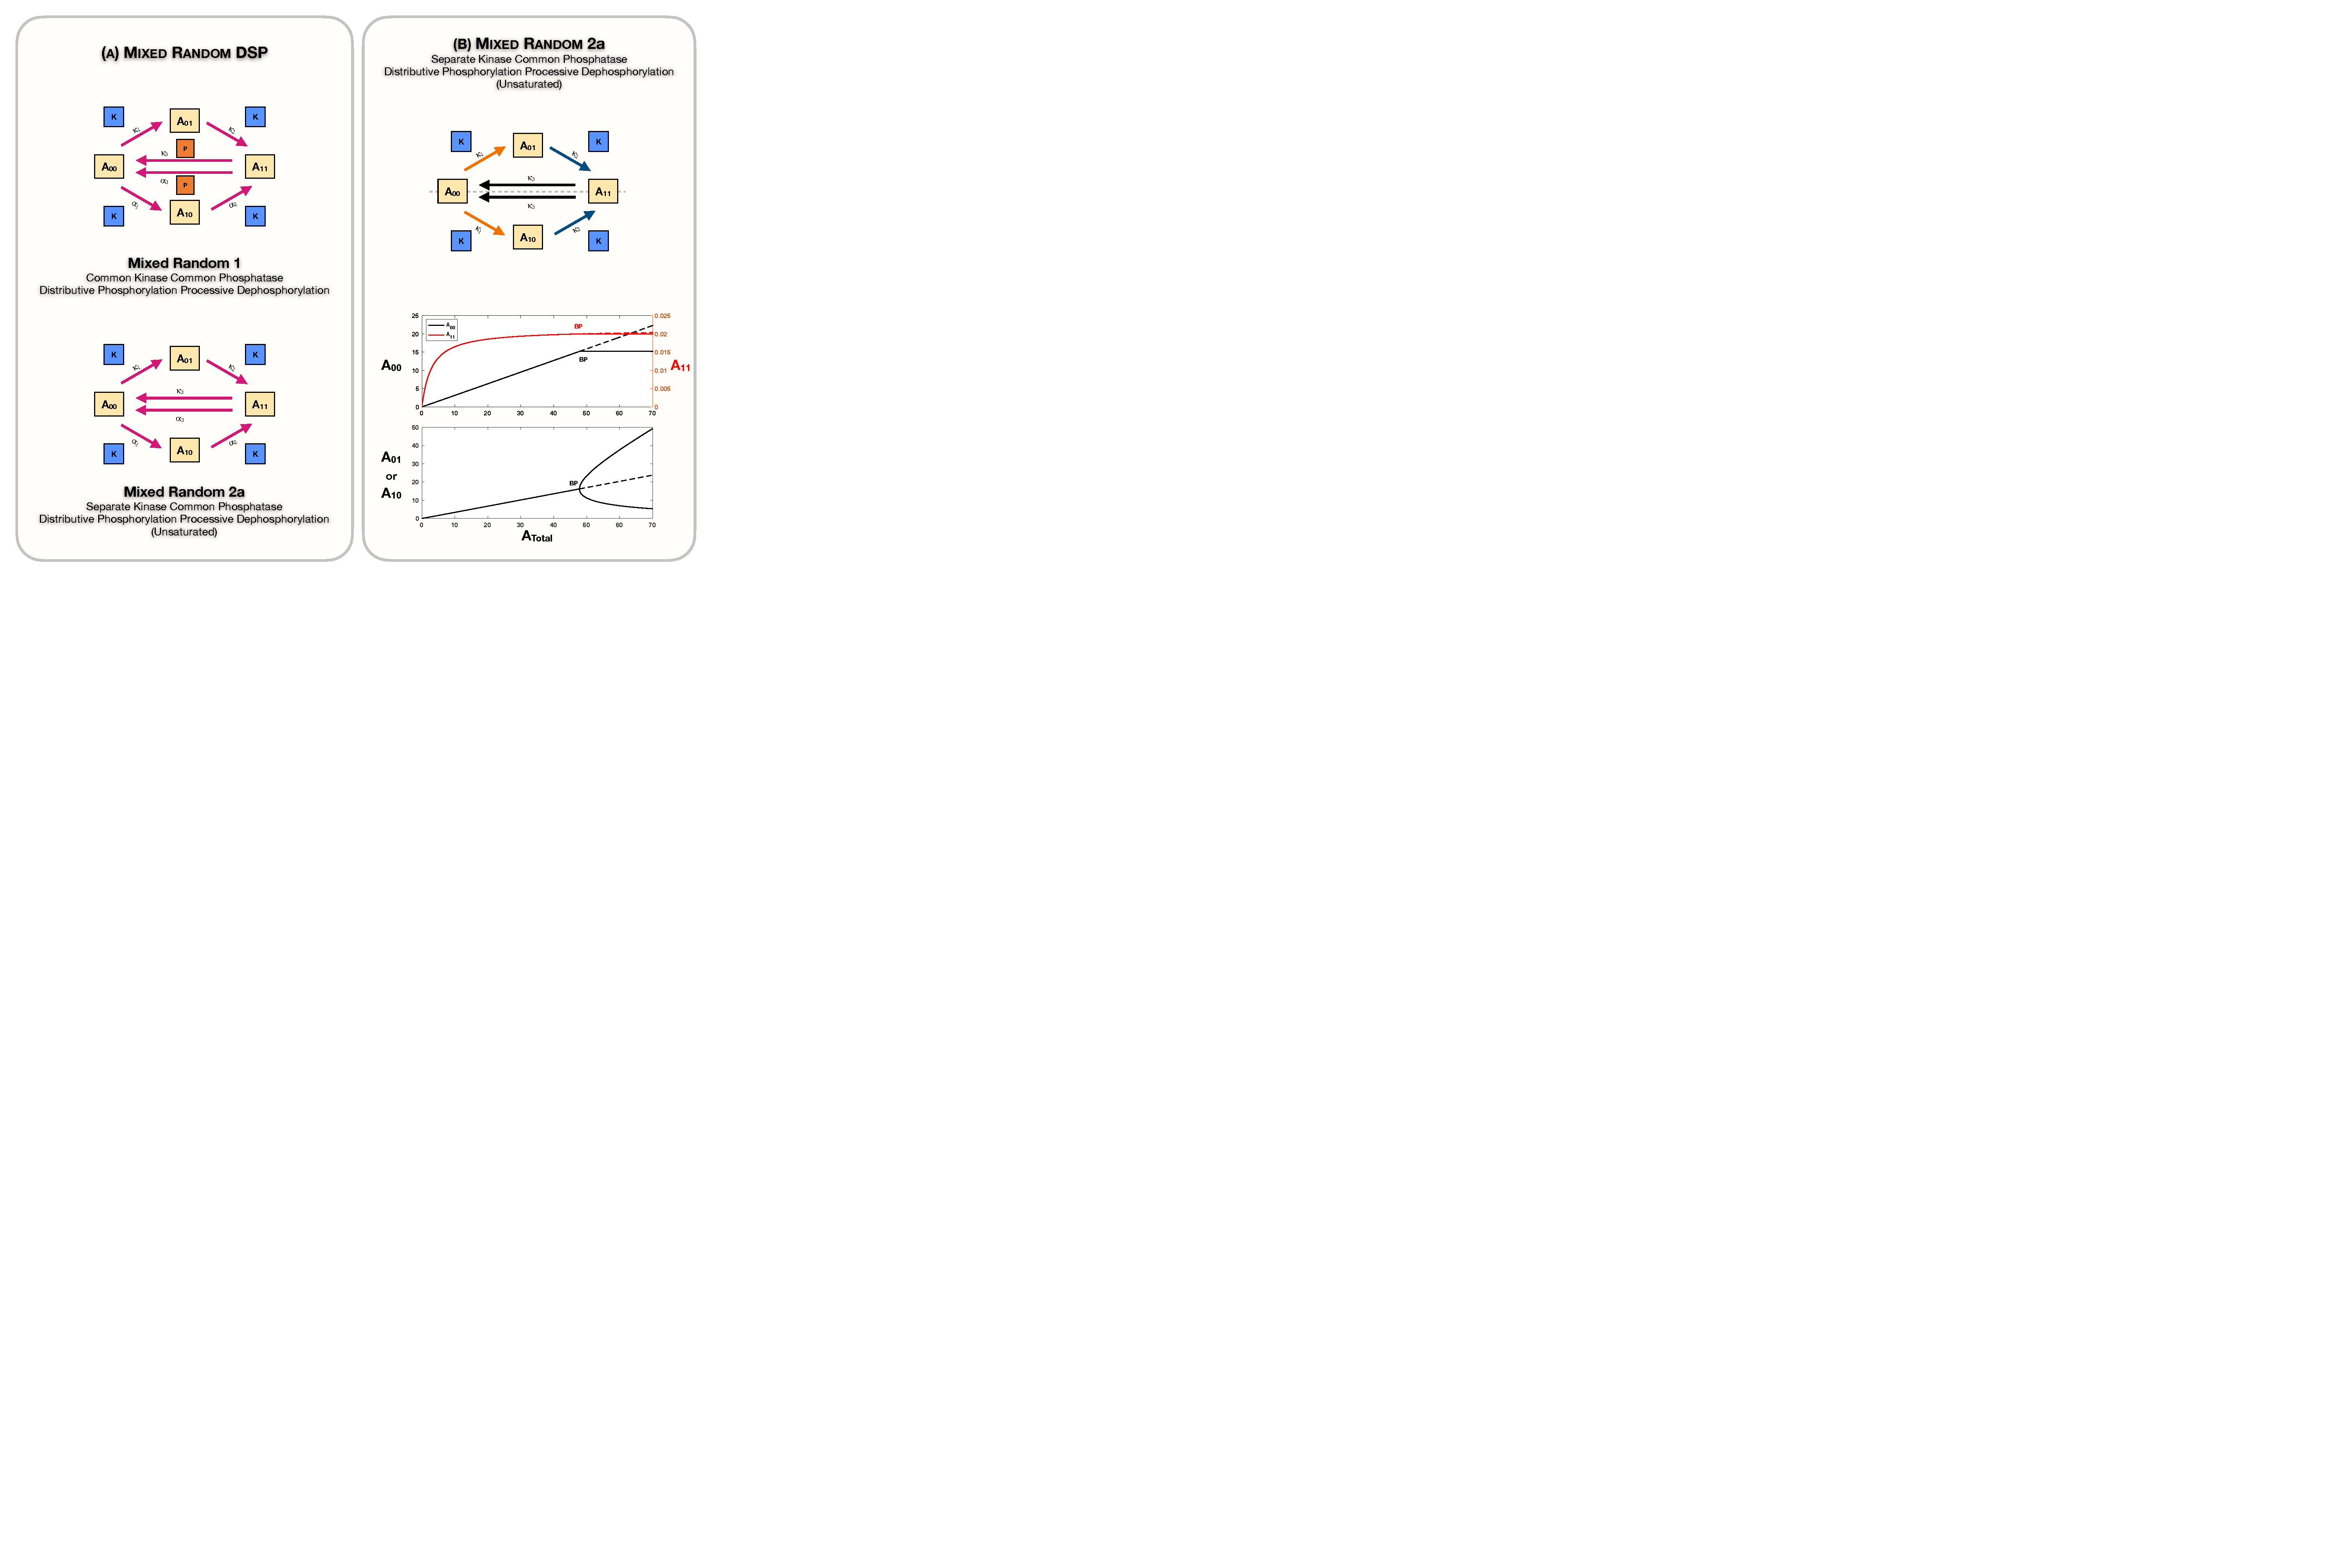
\includegraphics[width = 0.9\textwidth, keepaspectratio]{Supplementary_Figures/FigS01.pdf}
    \caption{(A). Schematic representation of the mixed random ordered DSP network with common kinase and common phosphatase effecting distributive  phosphorylation and processive dephosphorylation (Mixed Random 1), and the mixed random ordered DSP network with separate kinases and common phosphatase effecting distributive phosphorylation and processive dephosphorylation in the unsaturated regime (Mixed Random 2a). (B) shows case 2 symmetry breaking in the Mixed Random 2a network. Note that the concentration of the fully modified and unmodified substrate forms are fixed in the asymmetric steady states.
    [Dotted lines indicate unstable steady states, while solid lines represent stable steady states in the bifurcation diagram. BP: Pitchfork bifurcation]}
    \label{Fig S1}
\end{figure}

\clearpage
\begin{figure}[ht!]
    \centering
    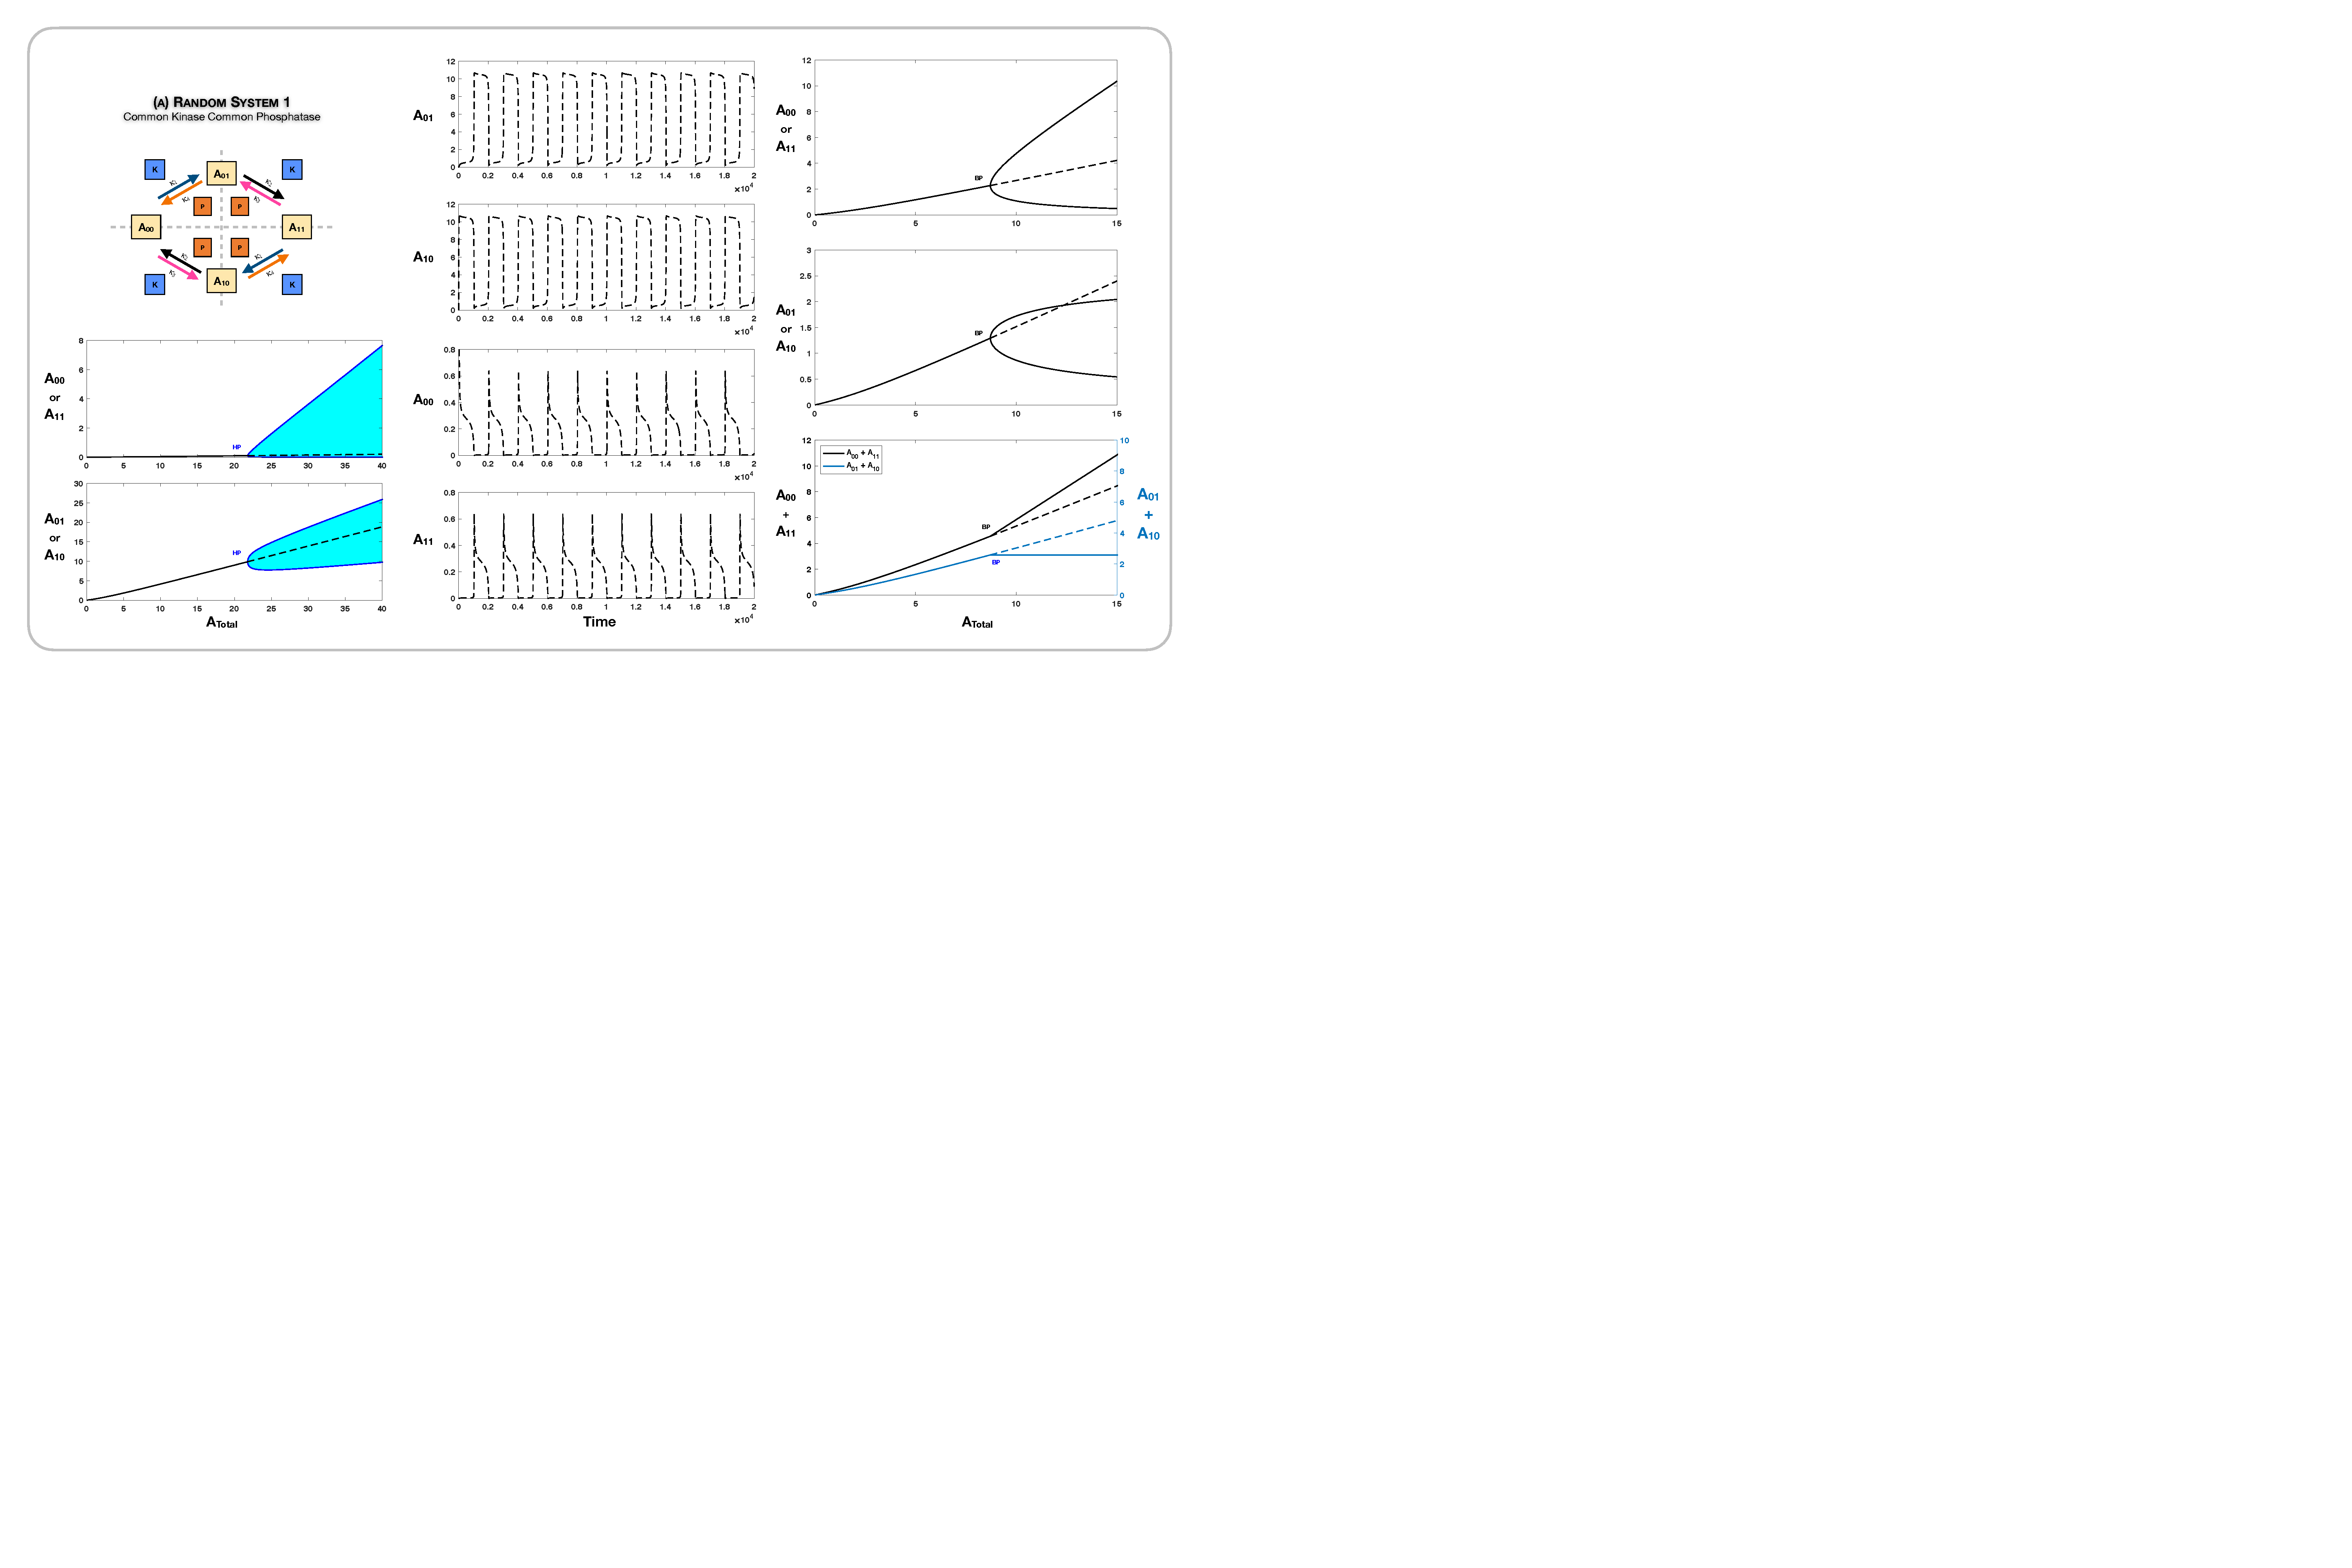
\includegraphics[width = 0.9\textwidth, keepaspectratio]{FigS02.pdf}
    \caption{Case 3 symmetry breaking in random ordered DSP with common kinase and common phosphatase acting on each modification site.
    Column 1 shows the presence of oscillations emerging through a Hopf bifurcation in the bifurcation diagram along $A_{Total}$. 
    Column 2 shows long period oscillations in the system represented in \Cref{Fig 3}(A) from the main text (for a $A_{Total} = 12.95$). Such long period oscillations emerge when the oscillatory branch from the Hopf bifurcation approaches asymmetric stable steady states.  
    Column 3 shows the presence of symmetry breaking through a supercritical Pitchfork bifurcation. Note that the sum of concentrations of the partial substrates is conserved in the asymmetric steady states. This network is also capable of symmetry breaking through a subcritical pitchfork as seen in \cref{Fig 3}.
    [Dotted lines indicate unstable steady states, while solid lines represent stable steady states in the bifurcation diagram. Shaded regions in the bifurcation diagram indicate regions of oscillations and the blue lines indicate bounds on concentrations during such oscillations. BP: Pitchfork bifurcation, HP: Hopf bifurcation]}
    \label{Fig S2}
\end{figure}

\clearpage
\begin{figure}[ht!]
    \centering
    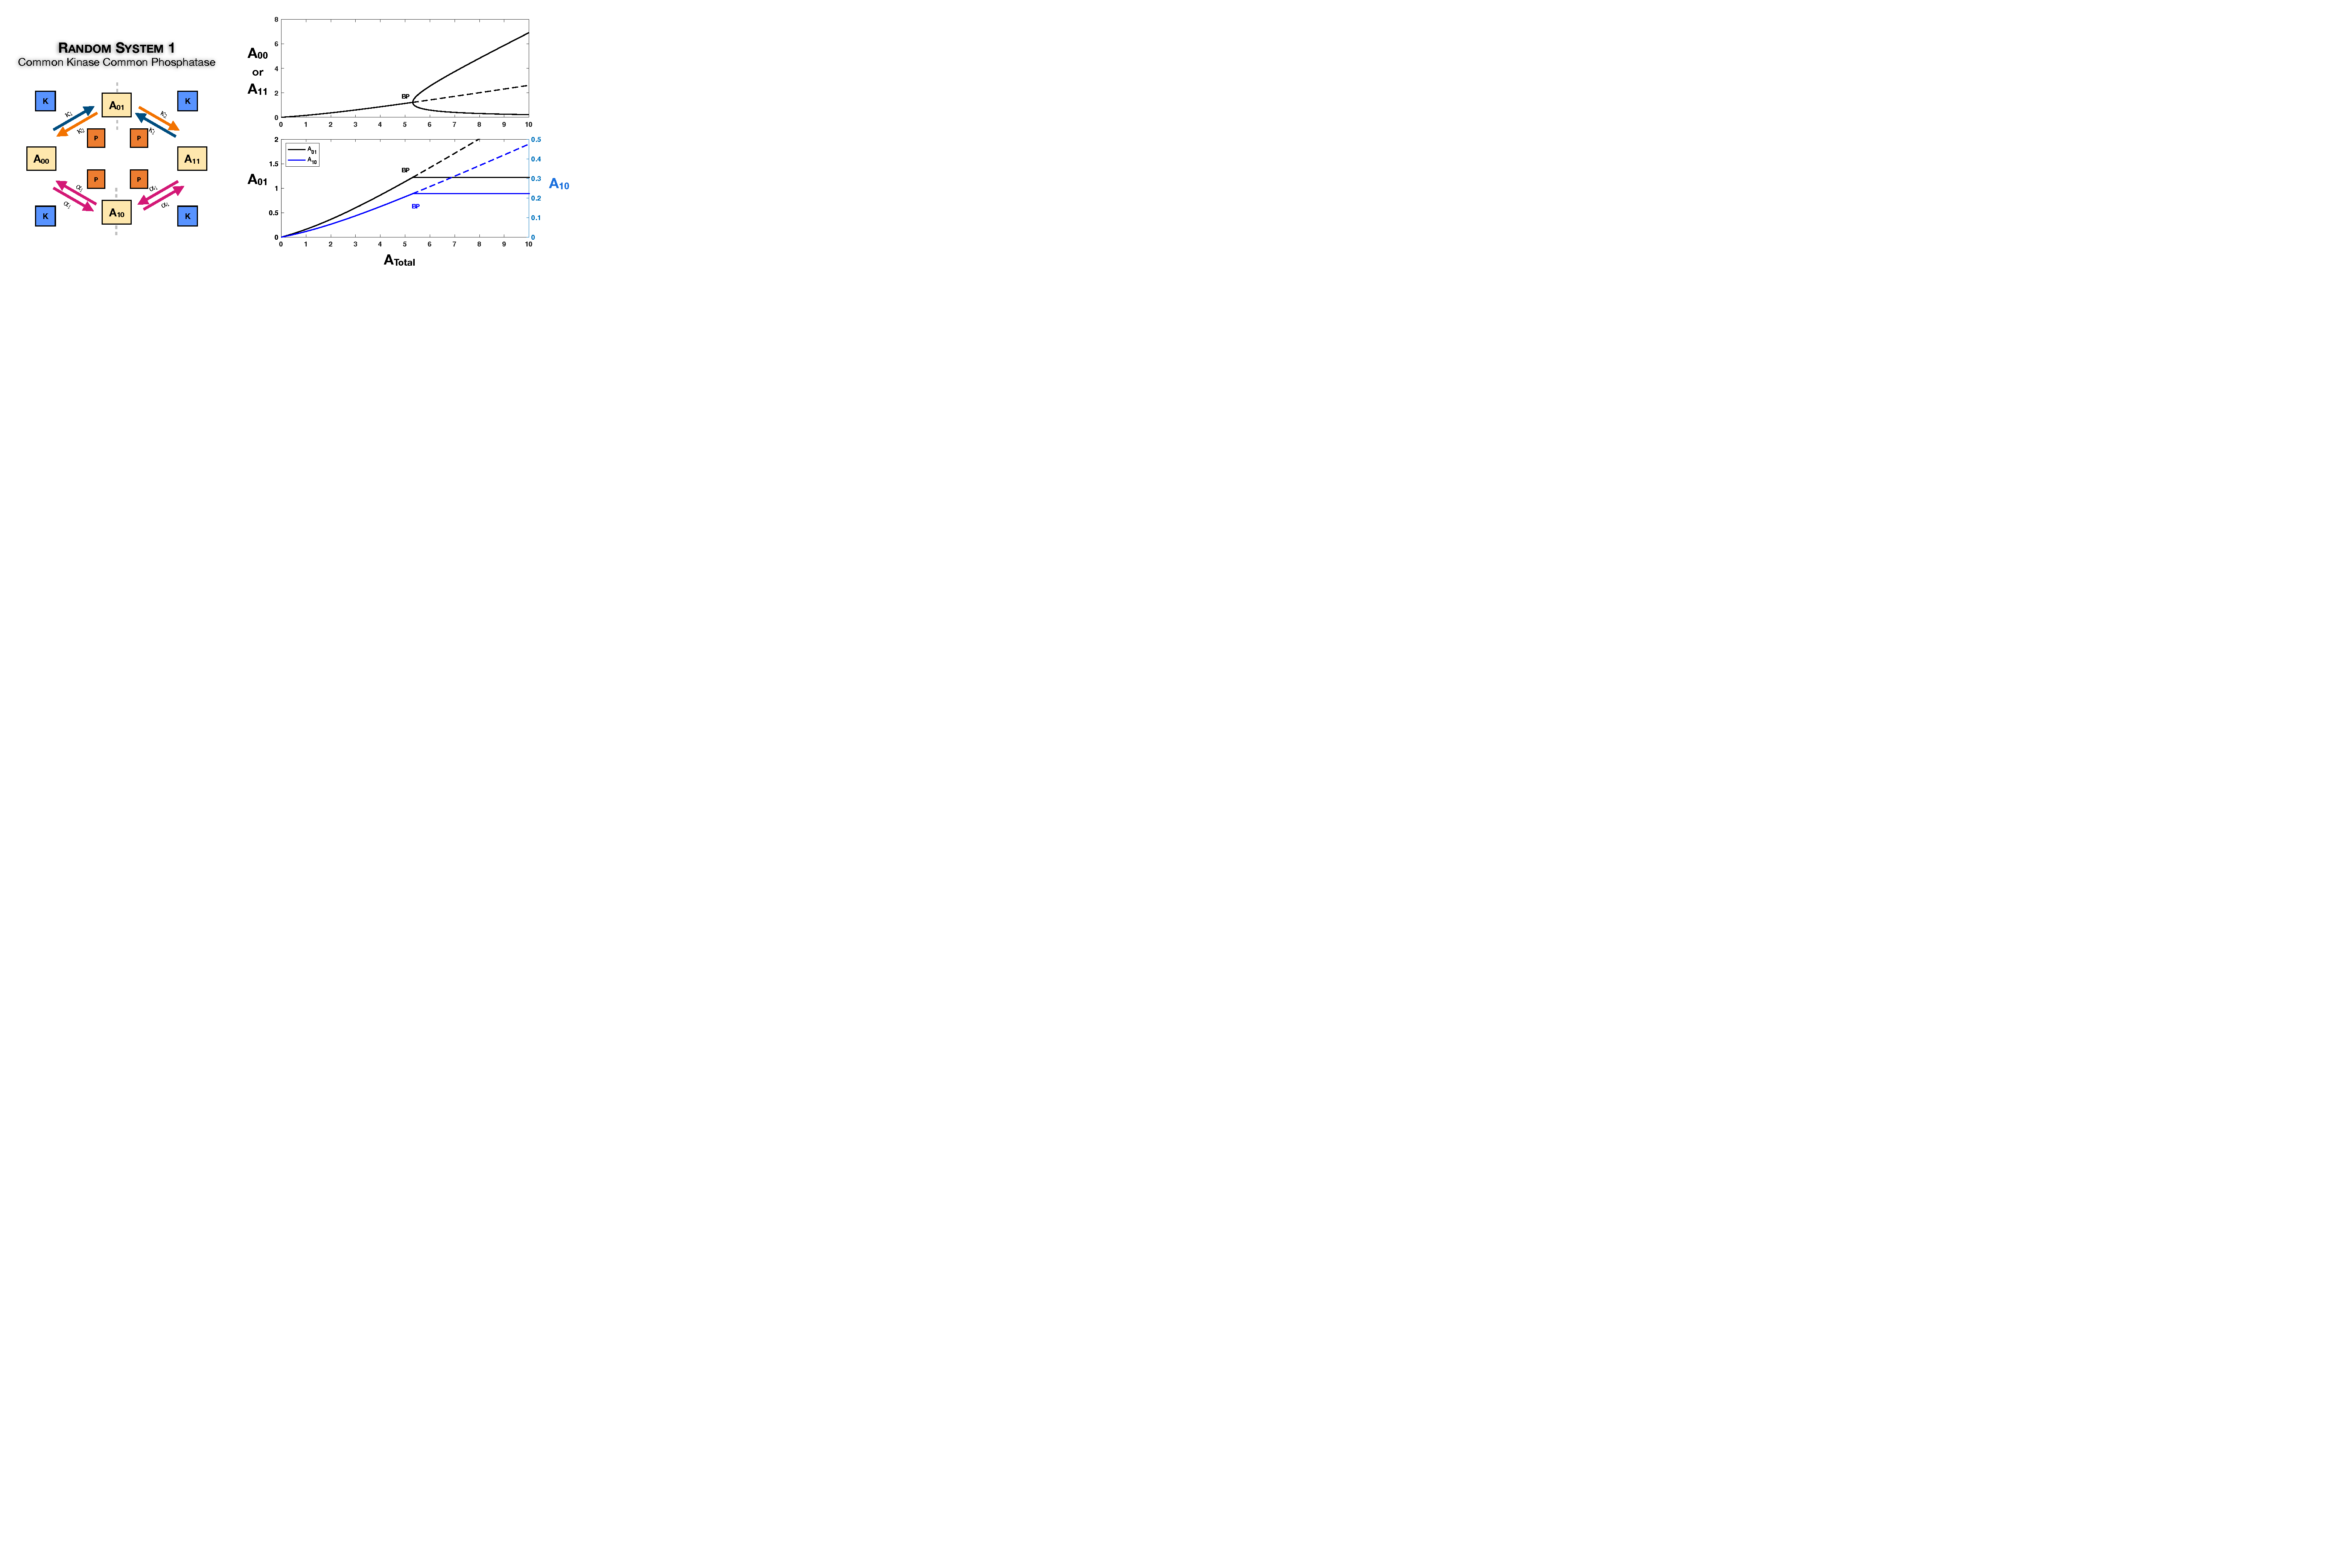
\includegraphics[width = 0.9\textwidth, keepaspectratio]{FigS03.pdf}
    \caption{Case 1 symmetry breaking in the random ordered DSP with common kinase and common phosphatase acting on each modification site, even when one of the legs ($A_{00} \Longleftrightarrow$ $A_{10} \Longleftrightarrow$ $A_{11}$) is incapable of breaking symmetry by itself (i.e. viewed as an ordered mechanism the kinetic parameters of the $A_{00} \Longleftrightarrow$ $A_{10} \Longleftrightarrow$ $A_{11}$ leg forbid independent symmetry breaking - see main text and analytical work for discussion). Homeostasis (Absolute Concentration Robustness) is observed in both partial substrates.
    [Dotted lines indicate unstable steady states, while solid lines represent stable steady states in the bifurcation diagram. BP: Pitchfork bifurcation]}
    \label{Fig S3}
\end{figure}

\clearpage
\begin{figure}[ht!]
    \centering
    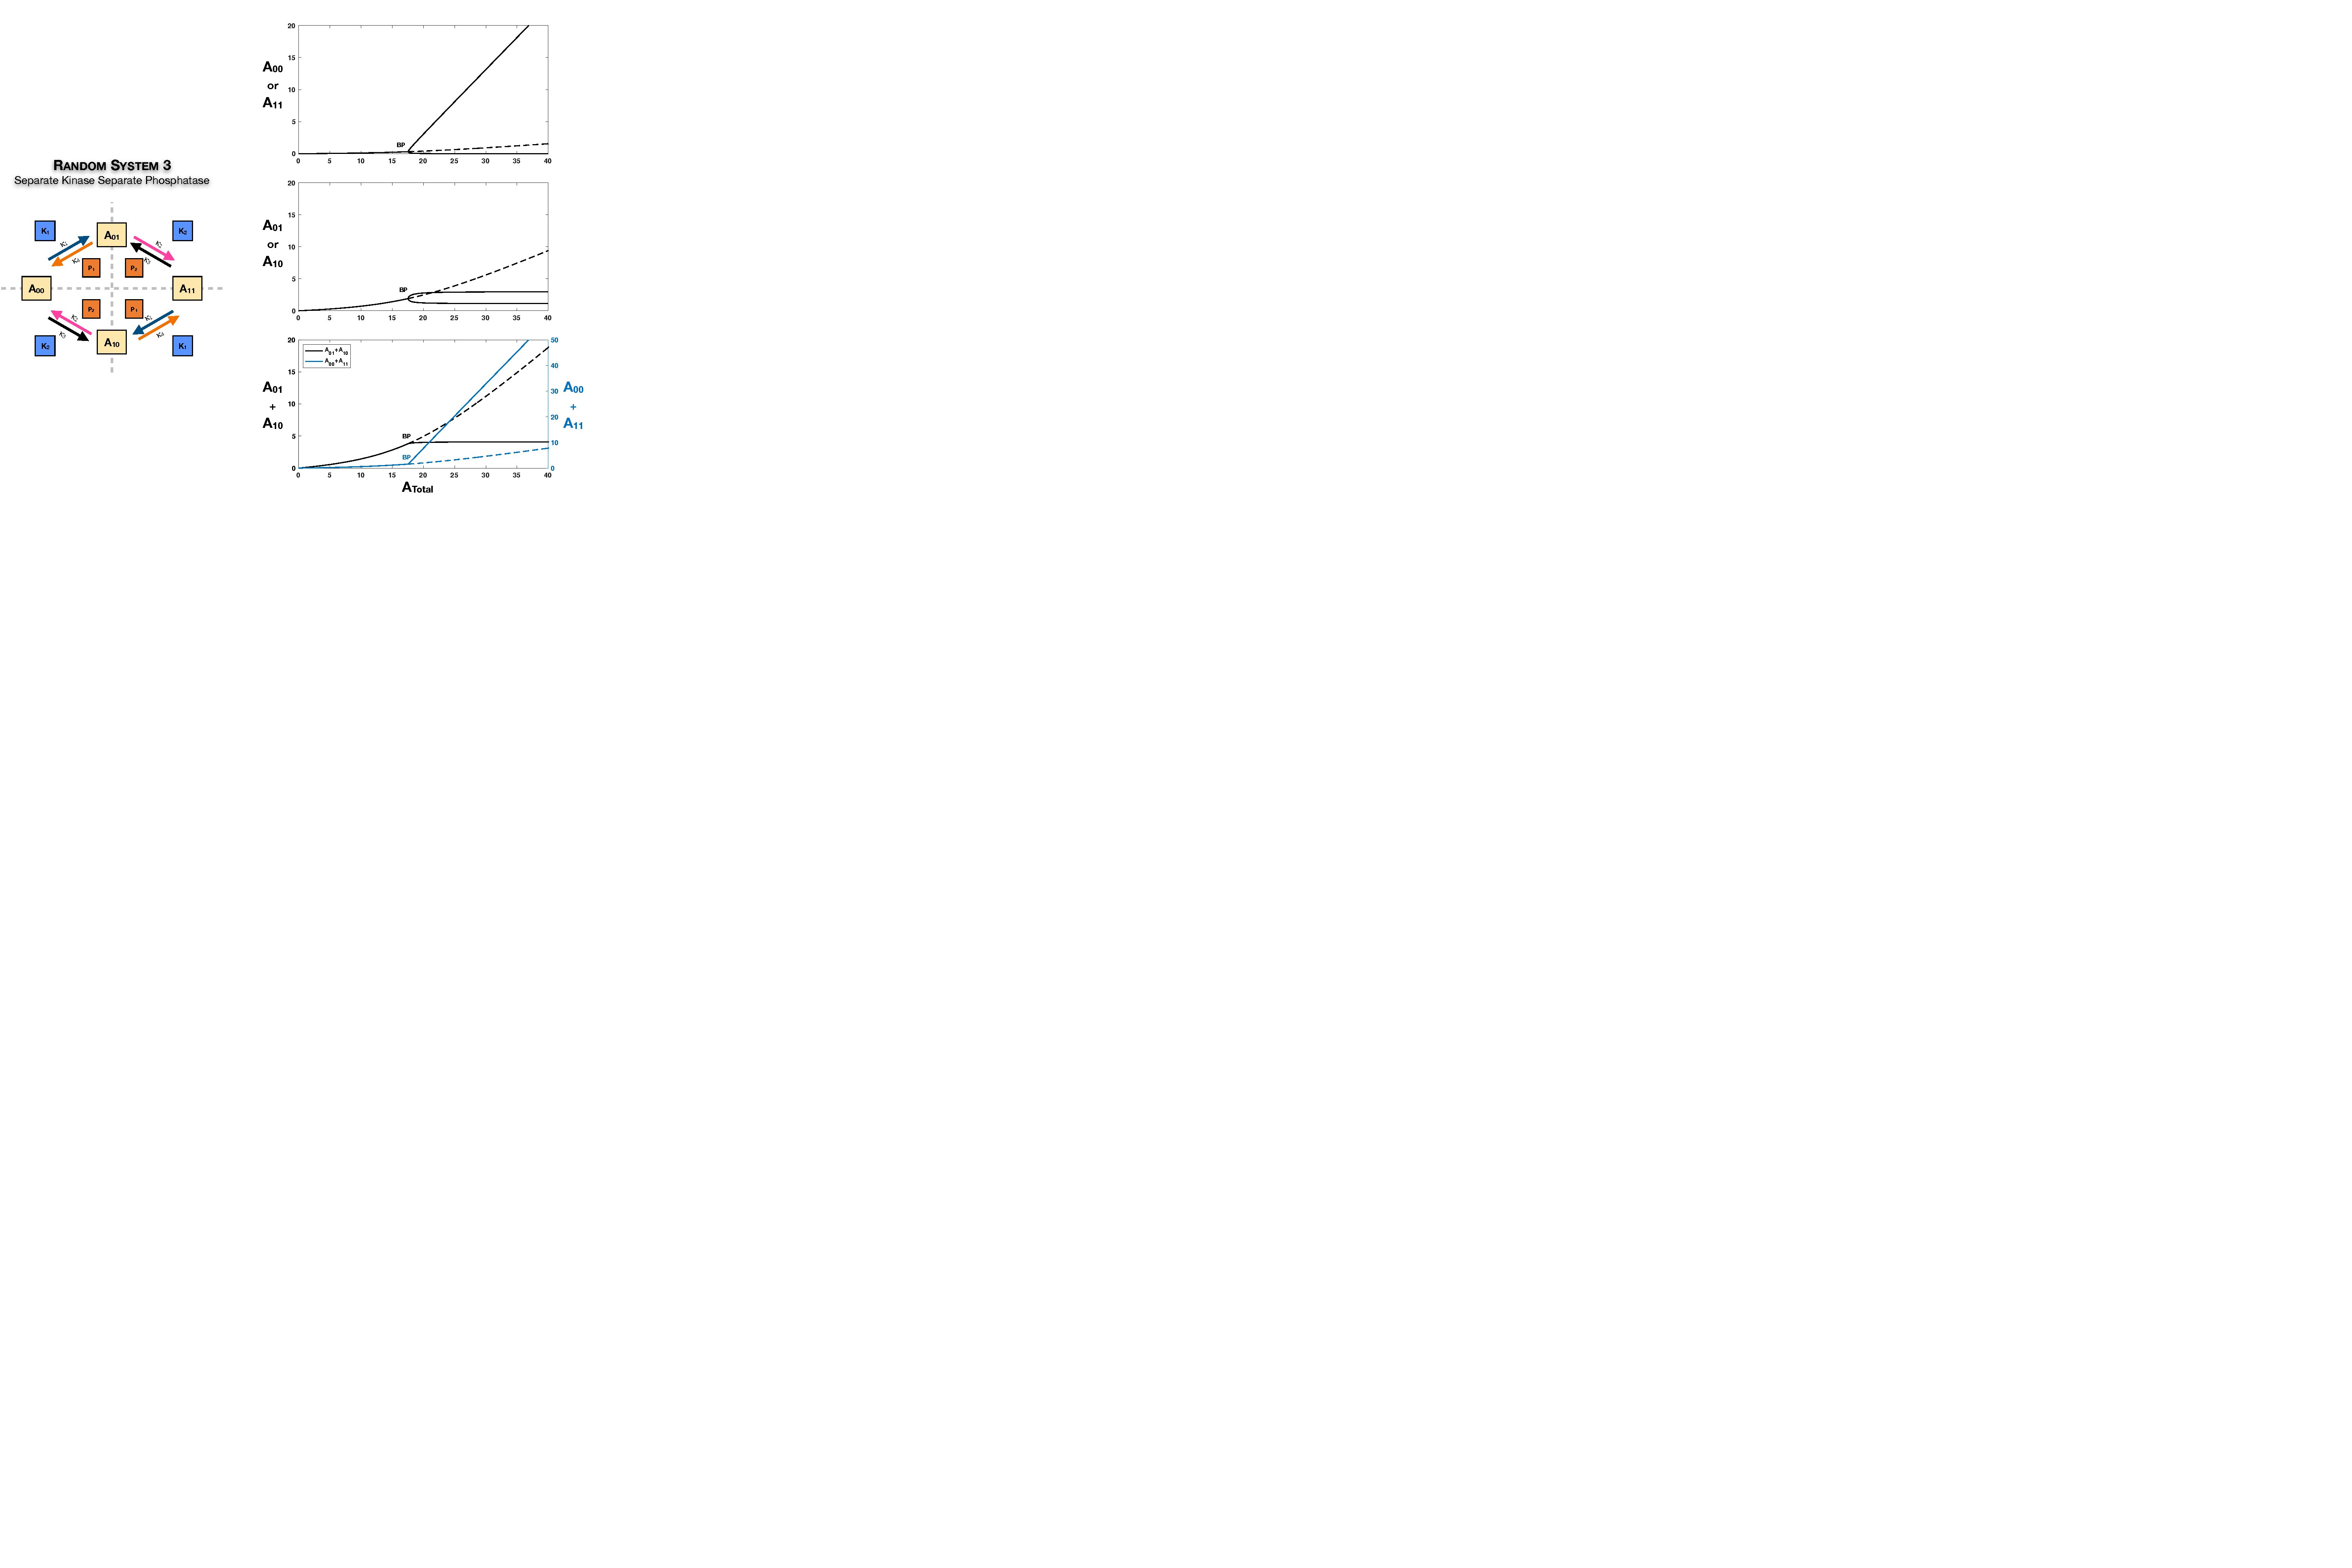
\includegraphics[width = 0.9\textwidth, keepaspectratio]{FigS04.pdf}
    \caption{Case 3 symmetry breaking through a supercritical pitchfork bifurcation in the random ordered DSP with separate kinase and separate phosphatase acting on each modification site. Note that the sum of the concentrations of the partially modified substrates is approximately fixed in the asymmetric steady states in the bifurcation diagram. However, case 3 symmetry breaking in this network is also capable of providing approximate concentration robustness in the sum of the concentrations of the completely modified and unmodified substrate forms - see main text and \cref{Fig 3}. [Dotted lines indicate unstable steady states, while solid lines represent stable steady states in the bifurcation diagram. BP: Pitchfork bifurcation]}
    \label{Fig S4}
\end{figure}

\clearpage
\begin{figure}[ht!]
    \centering
    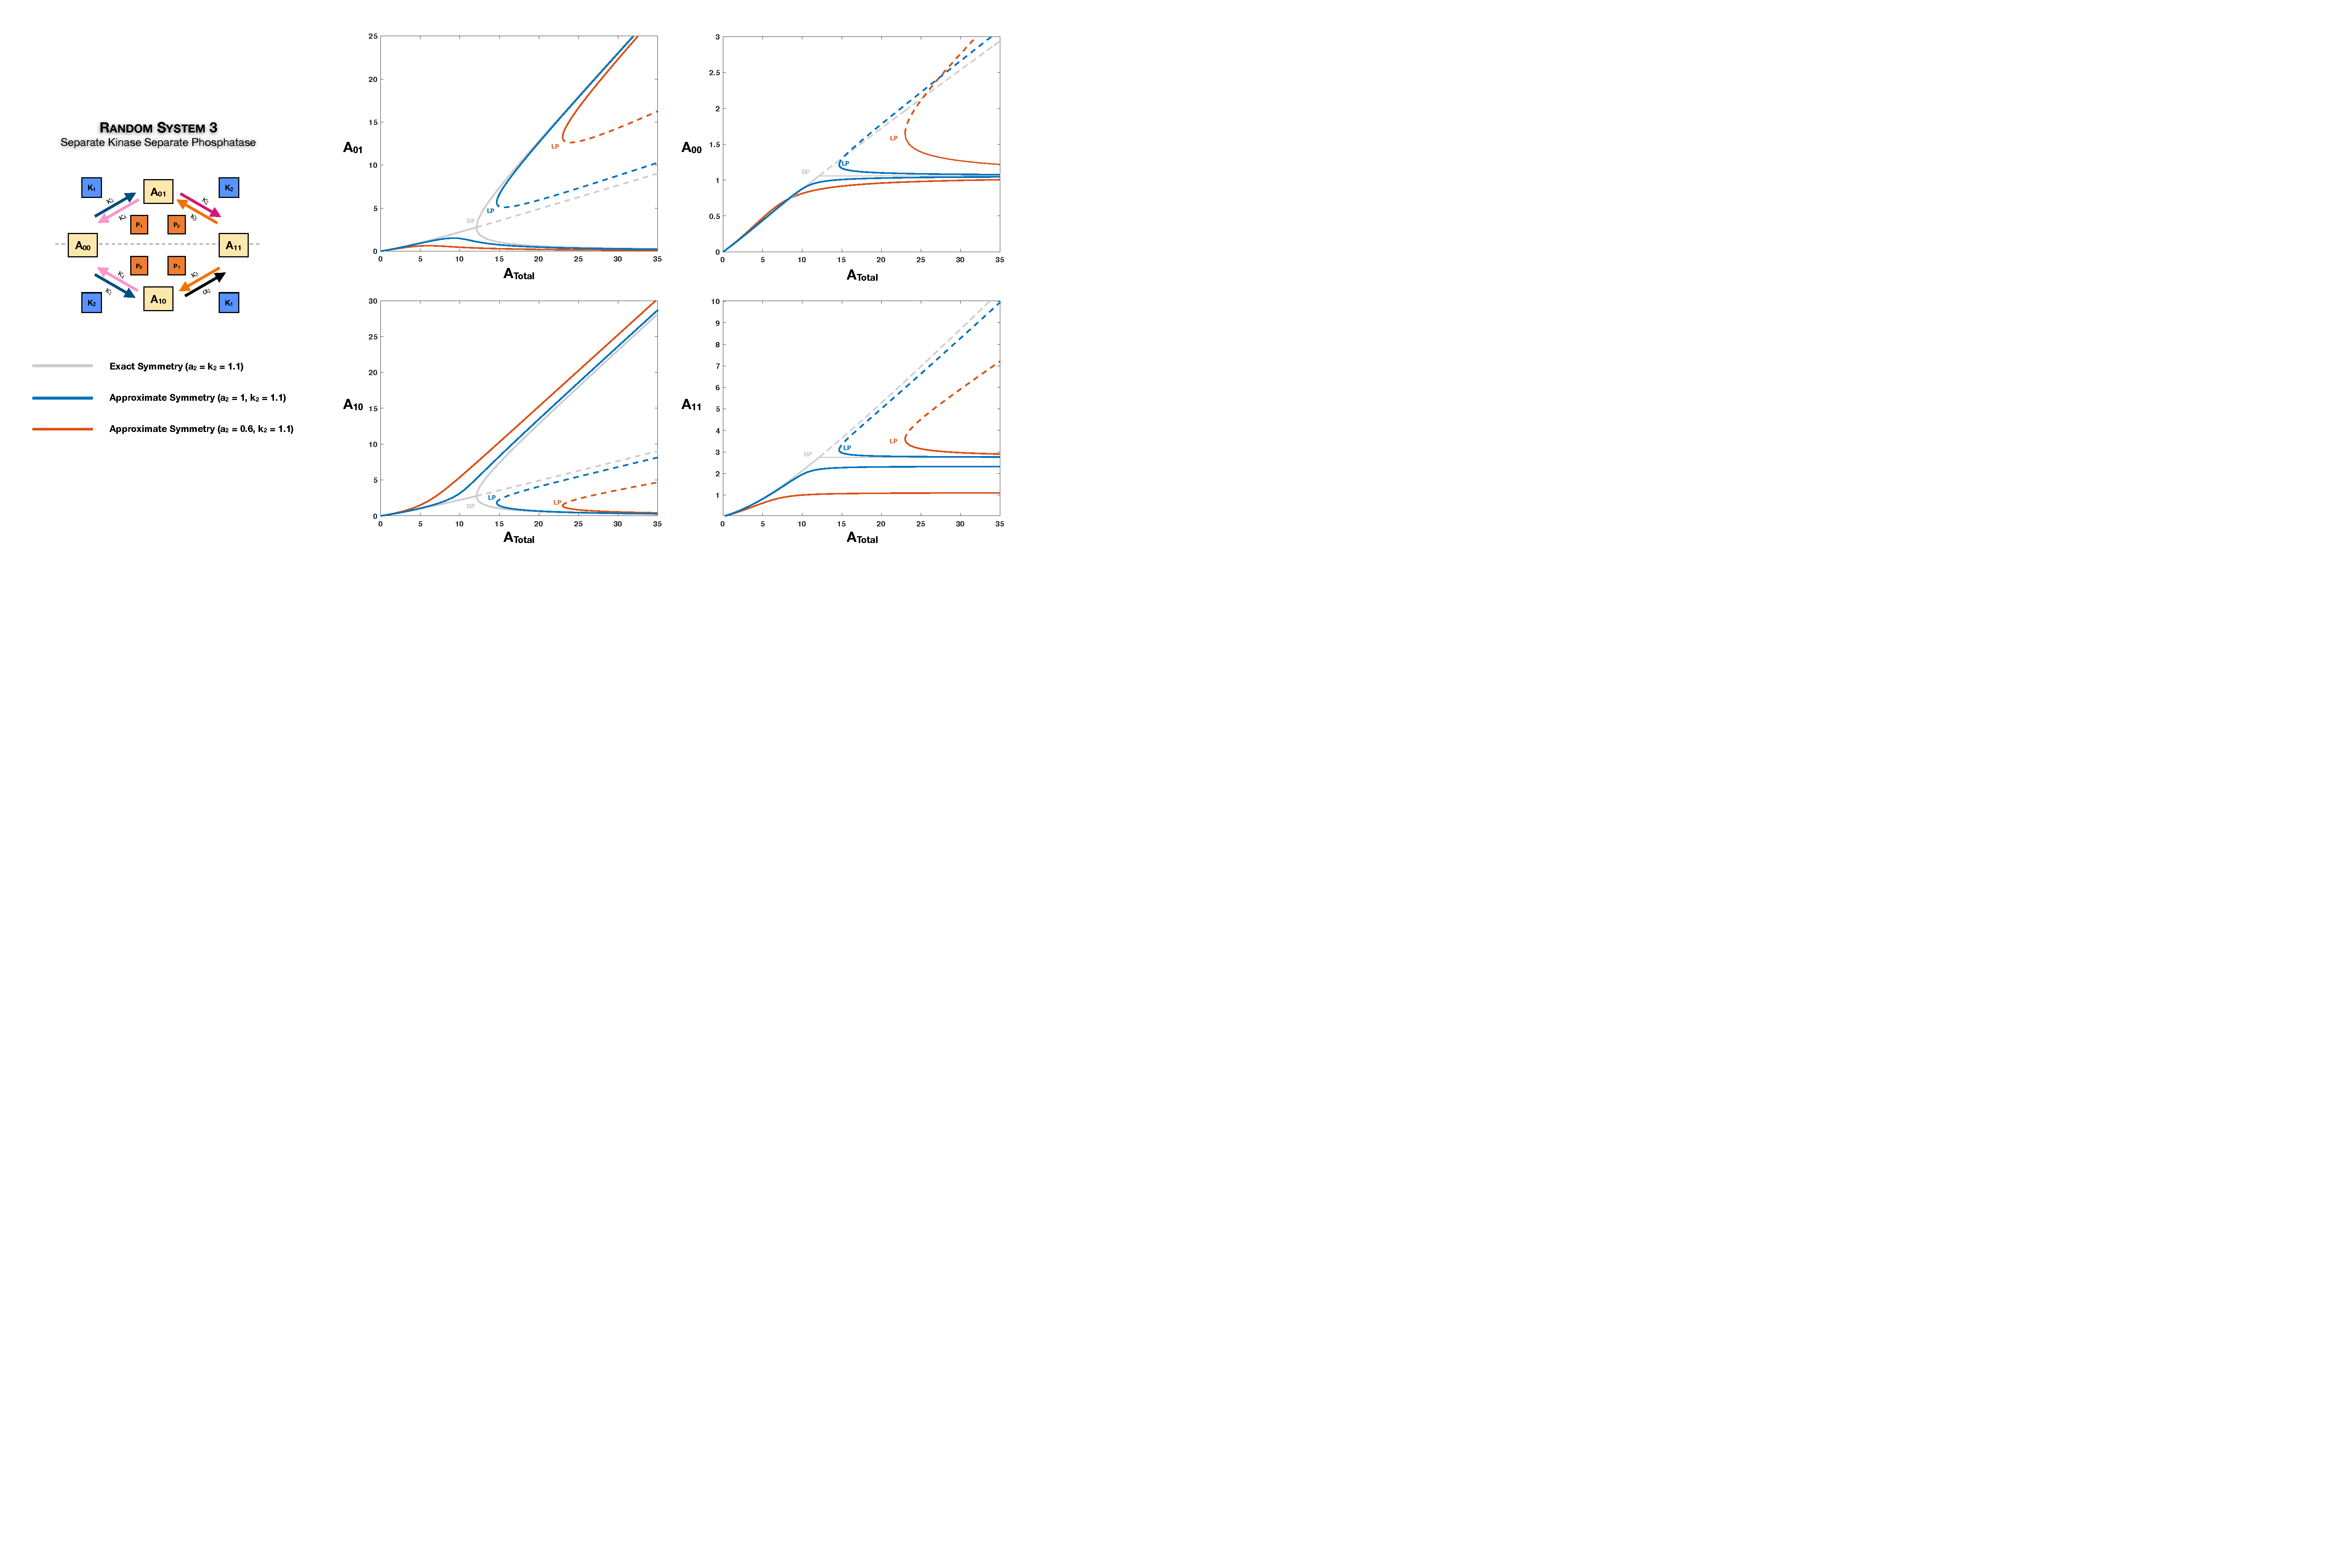
\includegraphics[width = 0.9\paperwidth, keepaspectratio]{Supplementary_Figures/FigS05.pdf}
    \caption{\textbf{Features of symmetry and symmetry breaking can still manifest when the network is only approximately symmetric.} This is represented through the example of case 2 symmetry breaking in the distributive ordered DSP with separate kinase and separate phosphatase affecting phosphorylation and dephosphorylation respectively. [Dotted lines indicate unstable steady states, while solid lines represent stable steady states in the bifurcation diagram. BP: Pitchfork bifurcation; LP: Saddle Node bifurcation]}
    \label{Fig S5}
\end{figure}

\clearpage
\begin{figure}
    \centering
    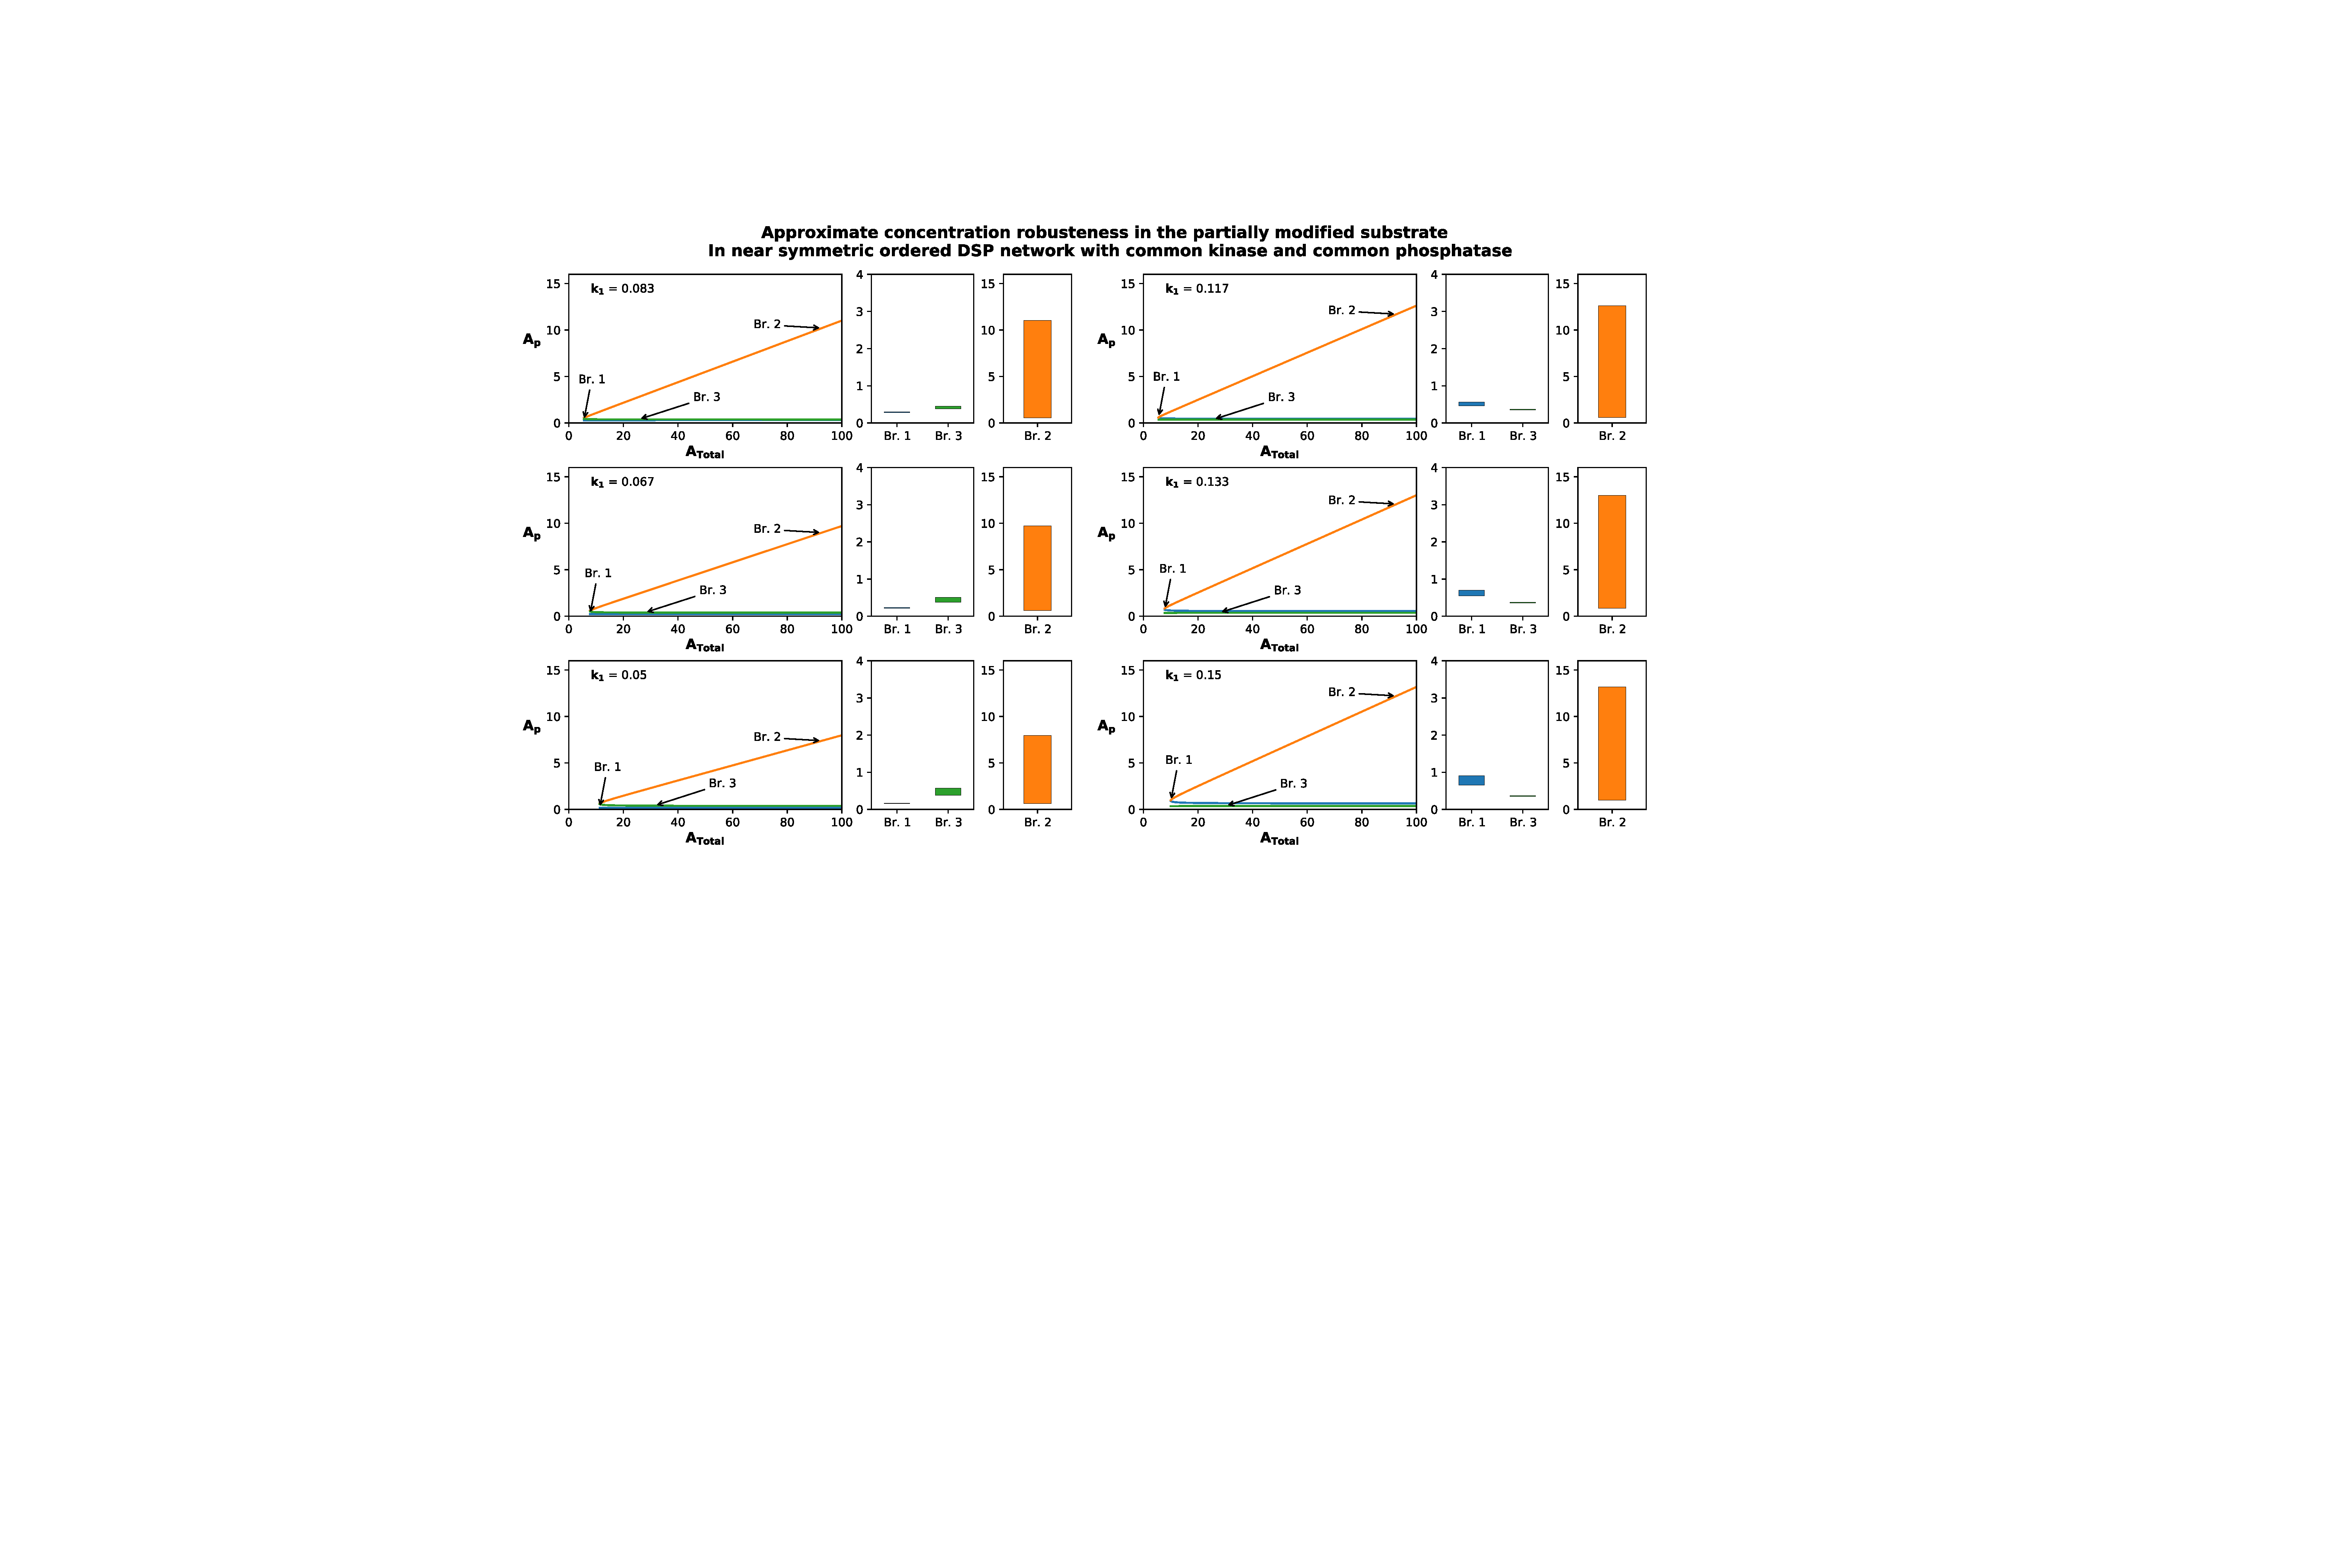
\includegraphics[width=0.9\paperwidth, height = 0.75\paperheight, keepaspectratio]{Supplementary_Figures/FigS06.pdf}
    \caption{\textbf{Approximate concentration robustness shown by systems that deviate from exact symmetry}: Figure represents the approximate concentration robustness shown by $A_p$ in the ordered distributive DSP with common kinase and common phosphatase when the network is not symmetric. Note that the system is symmetric when $k_1=1$ and is presented in \cref{Fig 2}A. In order to ascertain the behavior of the system and in particular ACR characteristics of $A_p$, we perturb the kinetics ($k_1$) at 6 values between $50\%$ and $150\%$ of the symmetric value (while keeping all other kinetics fixed) and present the result in 6 panels composed of three plots each; The first represents a bifurcation diagram showing the presence of steady state branches in a range of $A_{Total}$ (0 to 100) where multistability is present. The other two are bar graphs representing the norm of the concentration (Max value - Min value) of $A_p$ on the branches 1 and 3, and branch 2 respectively, across the entire range of variation ($A_{Total}=0- 100$). Note that in the symmetric network we obtain a perfect pitchfork bifurcation, however when the system deviates from exact symmetry, multistability is obtained through a saddle node bifurcation as shown here and in Appendix 2 - \cref{Fig S5}. The norm of $A_p$ is significantly smaller in magnitude on branches 1 and branches 3 (which would be the perturbed analogues of the ACR branches in the perfectly symmetric system) as compared to the norm in branch 2 (the perturbed analogue of the symmetric branch). The norm on branch 2 scales with increasing range of $A_{Total}$ (Note: the norm shown here is only for the range of $A_{Total} = 0 - 100$) while the norm of branches 1 and 3 are varying negligibly with changing $A_{Total}$. This behavior is depicted for 6 different parameter values between $50\%$ to $150\%$ and is again indicative of approximate concentration robustness seen in near symmetric systems for a large range of total substrate concentration.}
    \label{Fig S6}
\end{figure}

\clearpage
\begin{figure}[ht!]
    \centering
    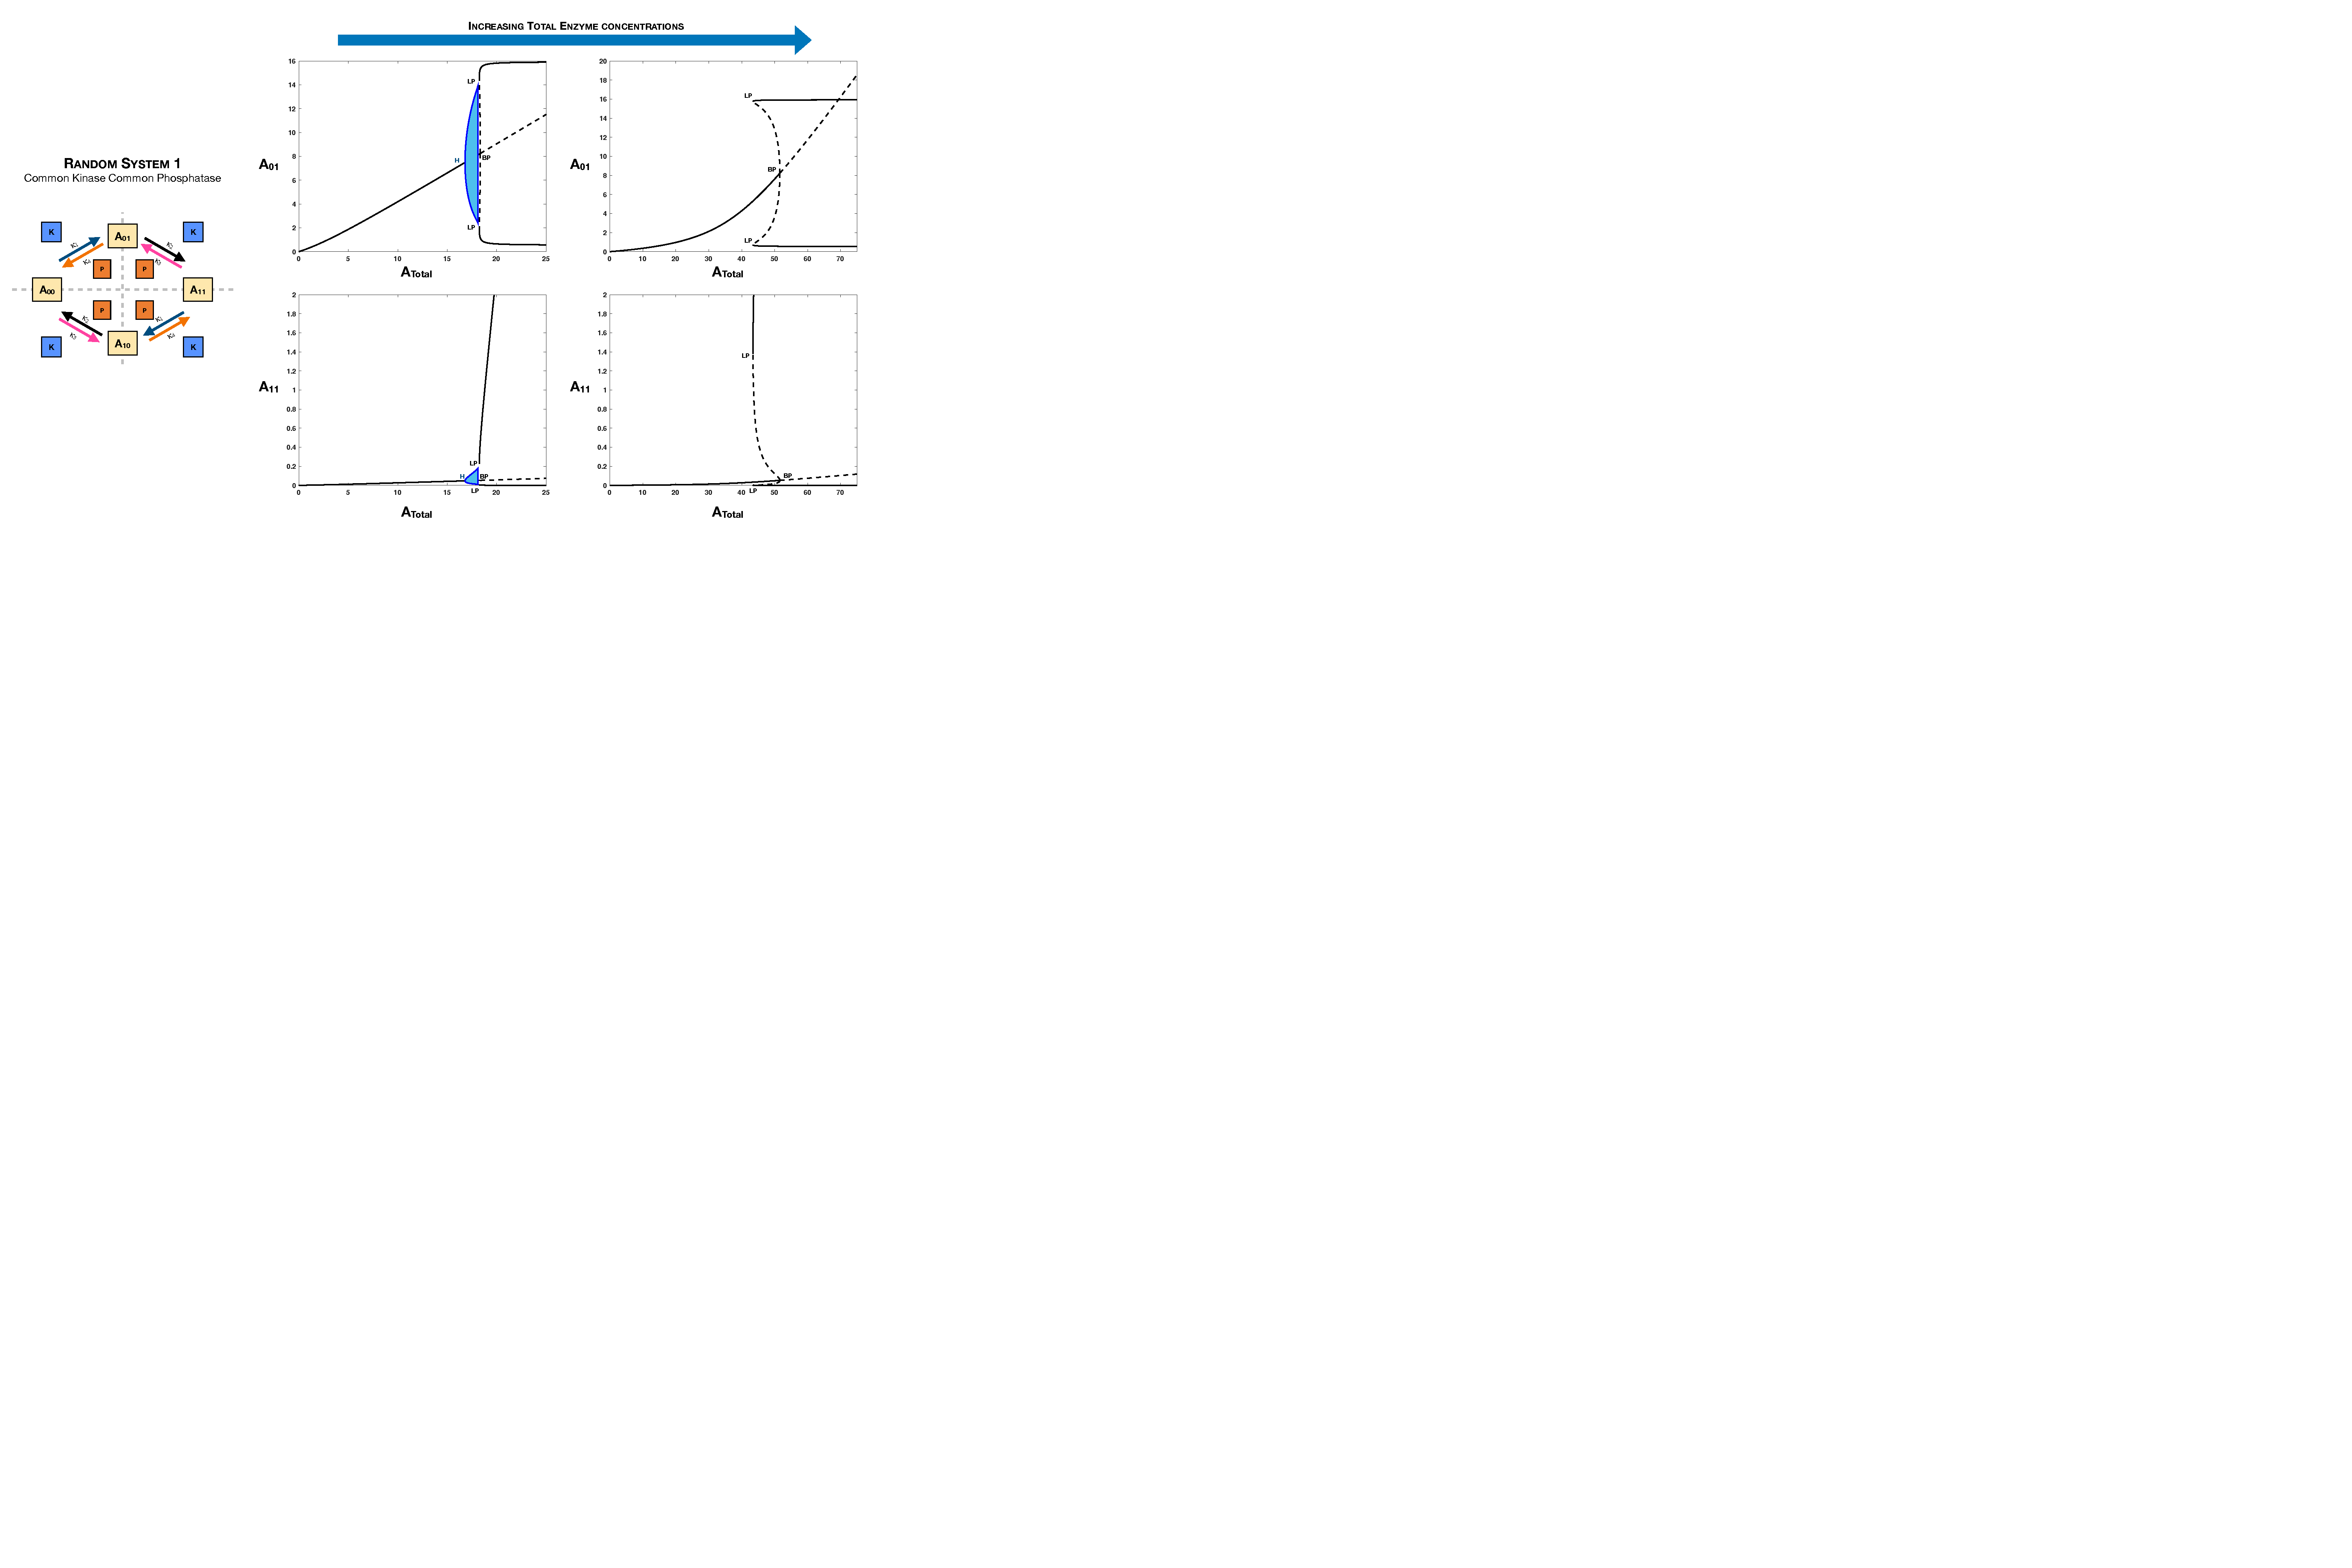
\includegraphics[width = 0.9\paperwidth, keepaspectratio]{Supplementary_Figures/FigS07.pdf}
    \caption{\textbf{Total enzyme concentrations are an additional lever (apart from basic network kinetics) that can independently tune symmetry breaking behavior in MSP networks.} This is represented through the example of case 3 symmetry breaking in the distributive random DSP with common kinase and common phosphatase). Panel 2 shows how increasing enzyme concentrations (left $\longrightarrow$ right) can lead to loss of oscillatory behavior in the network, for the same basal kinetics parameters.}
    \label{Fig S7}
\end{figure}

\clearpage
\begin{figure}
    \centering
    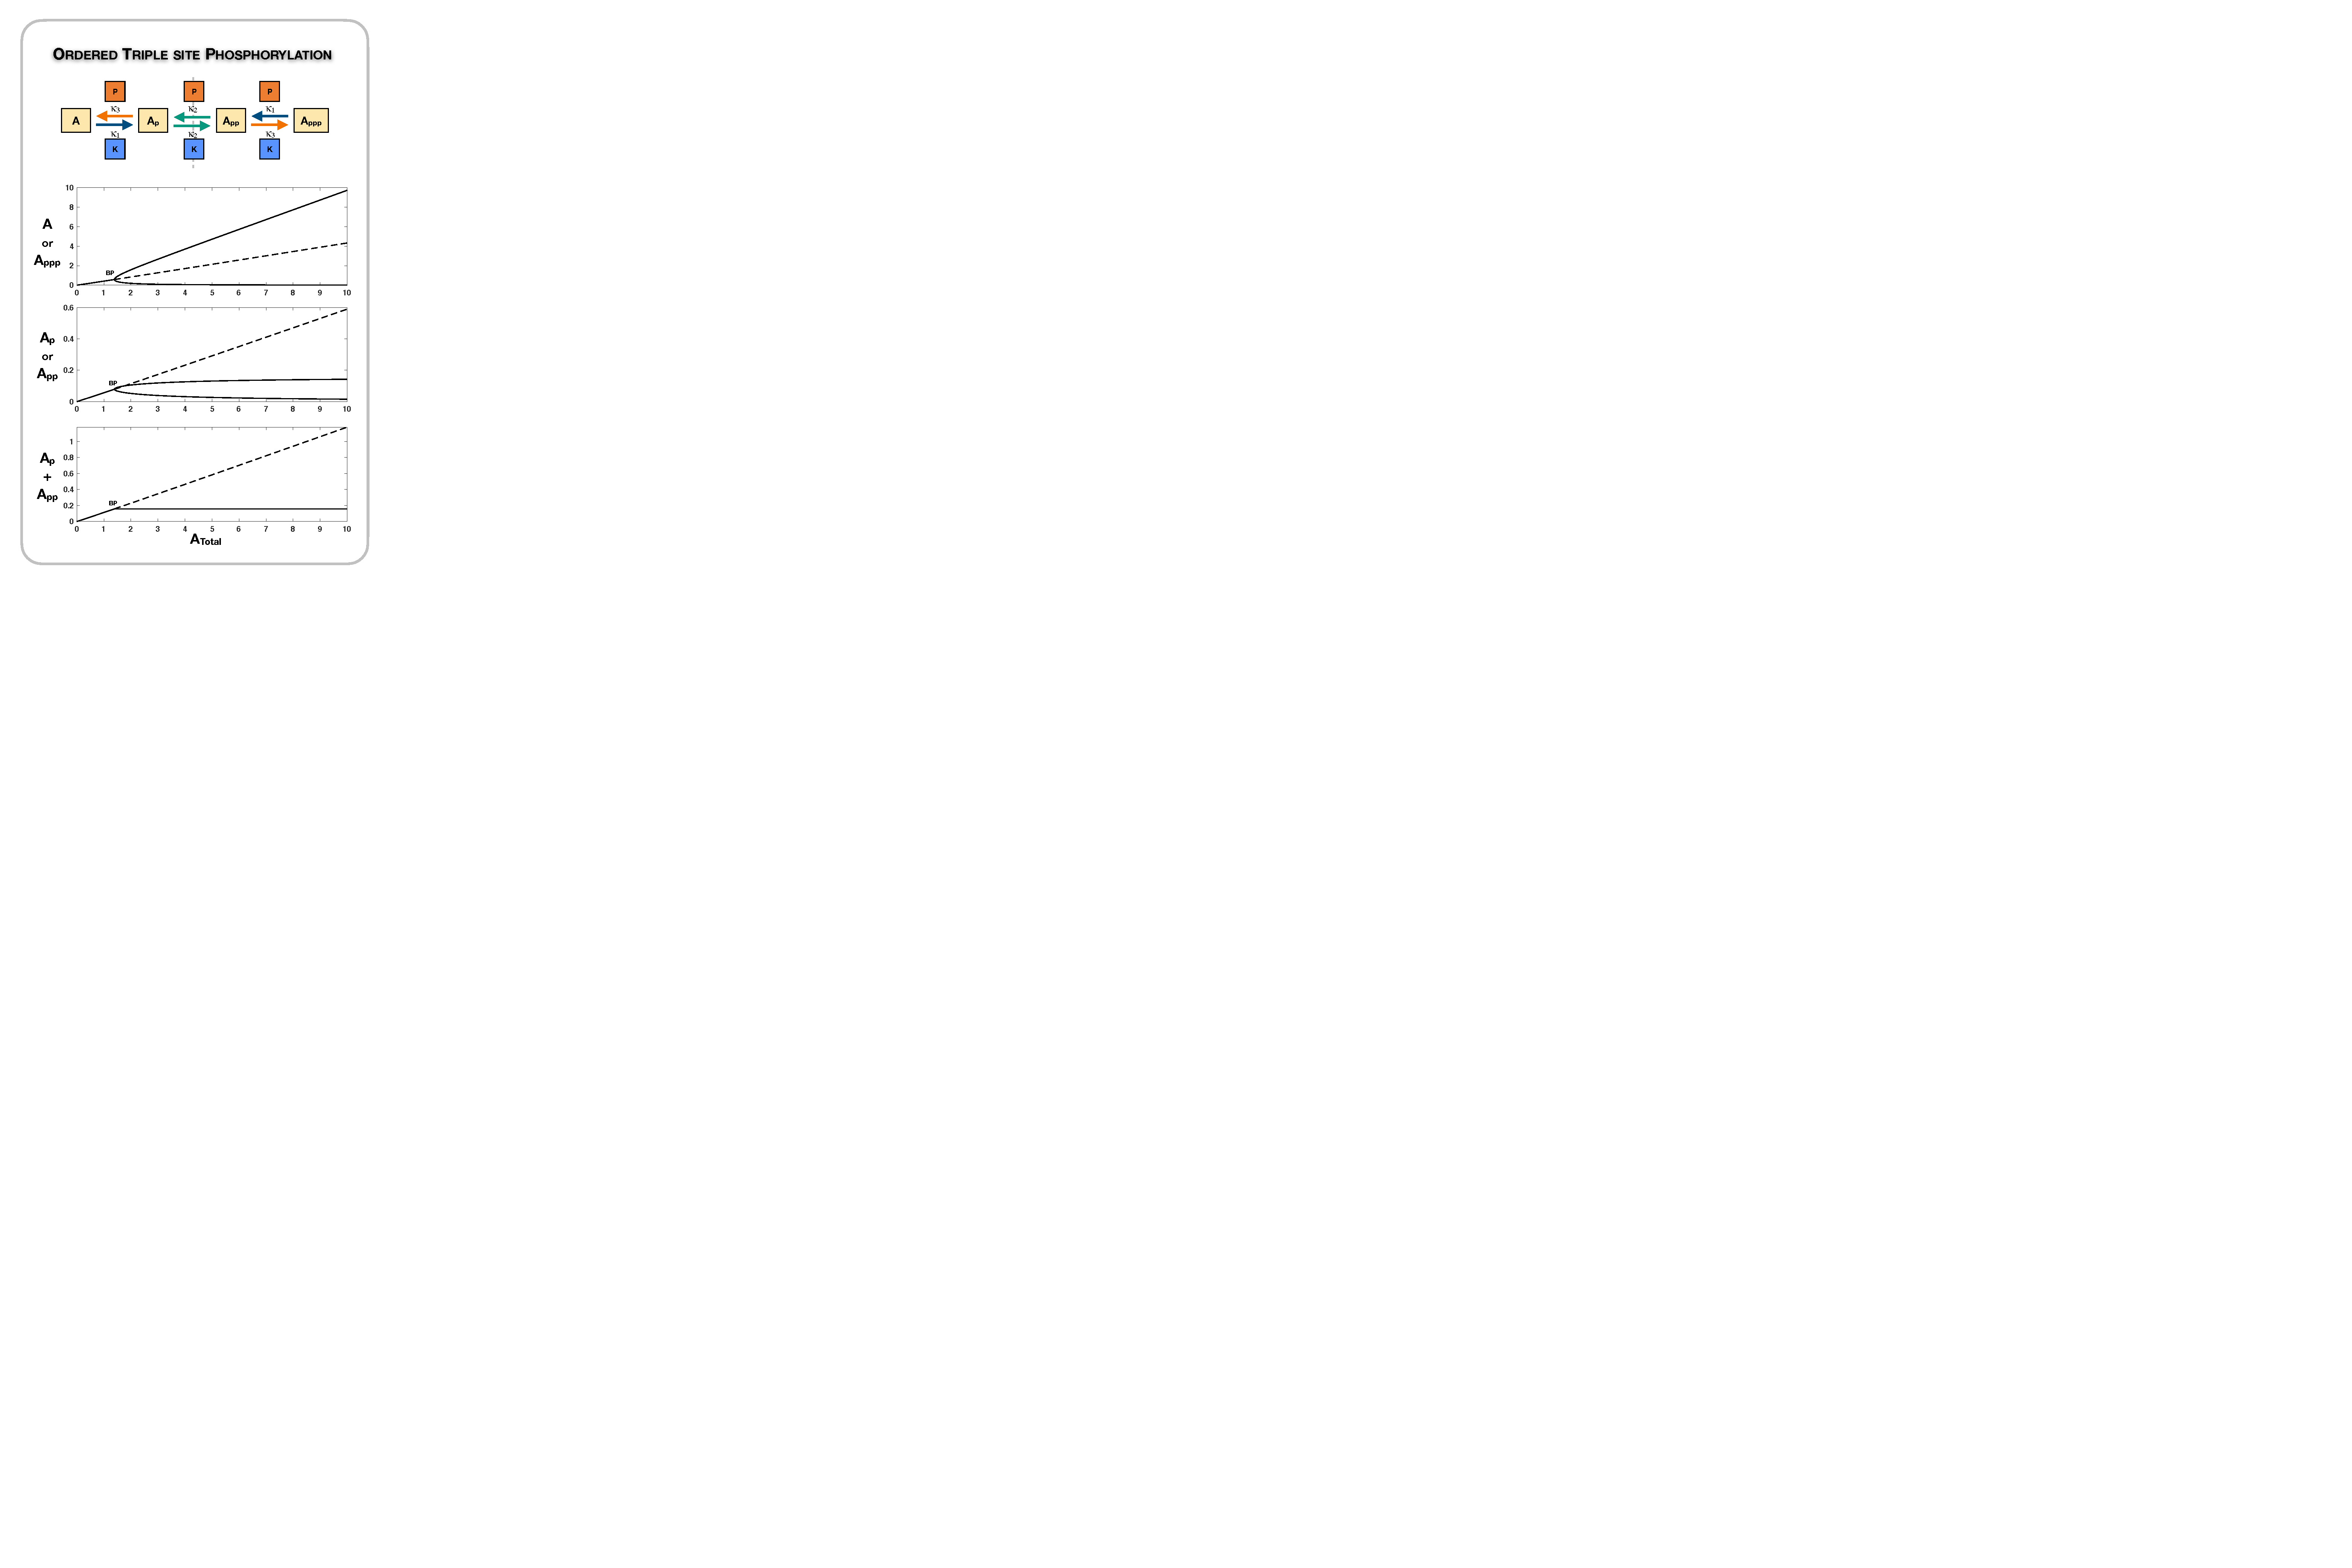
\includegraphics[width=0.9\paperwidth, height = 0.75\paperheight, keepaspectratio]{Supplementary_Figures/FigS08.pdf}
    \caption{Case 1 symmetry breaking in the distributive ordered TSP network. Here we observe Absolute Concentration Robustness in the sum of the concentrations of the partially modified substrates. [Dotted lines indicate unstable steady states, while solid lines represent stable steady states in the bifurcation diagram. BP: Pitchfork bifurcation]}
    \label{Fig S8}
\end{figure}

\clearpage
\begin{figure}[ht!]
    \centering
    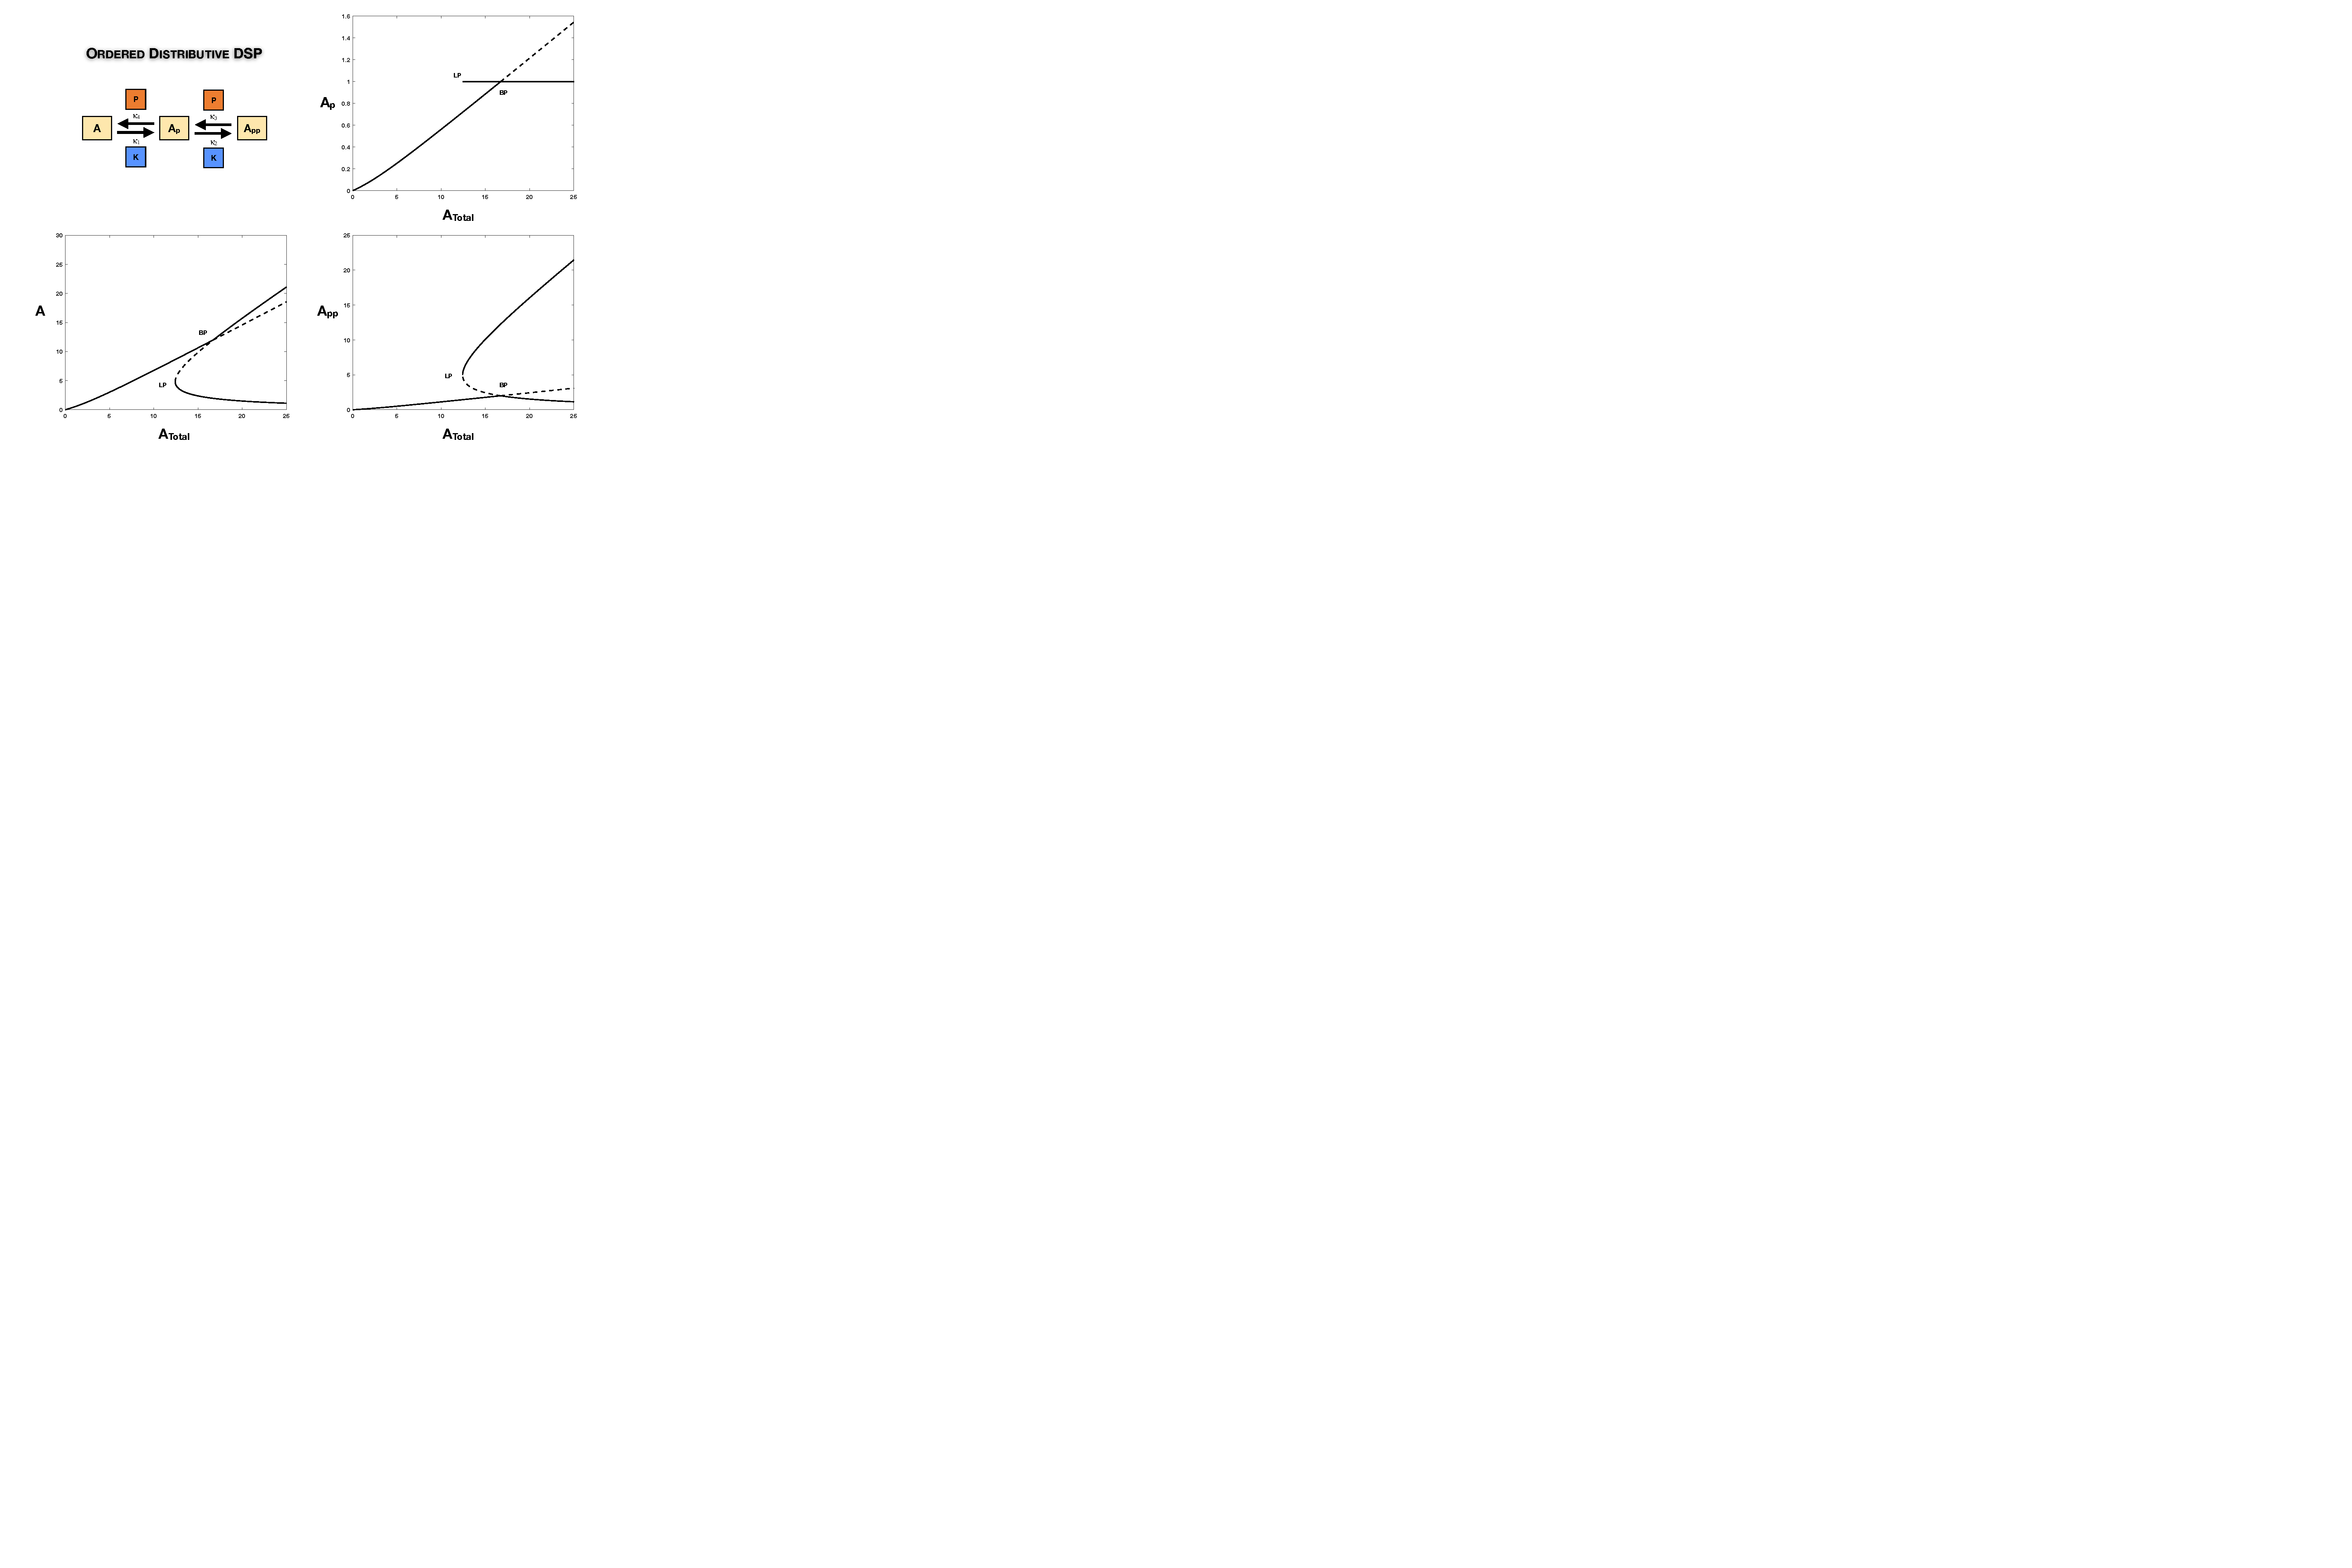
\includegraphics[width = 0.75\paperwidth, keepaspectratio]{Supplementary_Figures/FigS09.pdf}
    \caption{\textbf{Absolute Concentration Robustness in ordered DSP}: The ordered double site with common kinase common phosphatase is capable of exhibiting (exact) Absolute Concentration Robustness (ACR) in the partially modified substrate ($A_p$) with respect to changing total substrate concentration even in the absence of symmetry in the kinetics or total enzyme amounts (However a weaker constraint is required to enable this). The figure presents a computational example of this (complementing the discussion in the main text and the appendix 1). We observe a single non-ACR exhibiting branch of steady states exchanging stability with branches of ACR exhibiting steady states through a transcritical bifurcation (as opposed to a pitchfork bifurcation as seen in the symmetric examples earlier). The concentration of $A_p$ is fixed to be mathematically exact on these ACR branches as shown in the top-right plot. The unstable ACR branch emerging out of the transcritical bifurcation becomes stable through a saddle node bifurcation as shown. [Dotted lines indicate unstable steady states, while solid lines represent stable steady states in the bifurcation diagram. BP: Pitchfork bifurcation; LP: Saddle Node bifurcation]}
    \label{Fig S9}
\end{figure}

\clearpage
\begin{figure}[ht!]
    \centering
    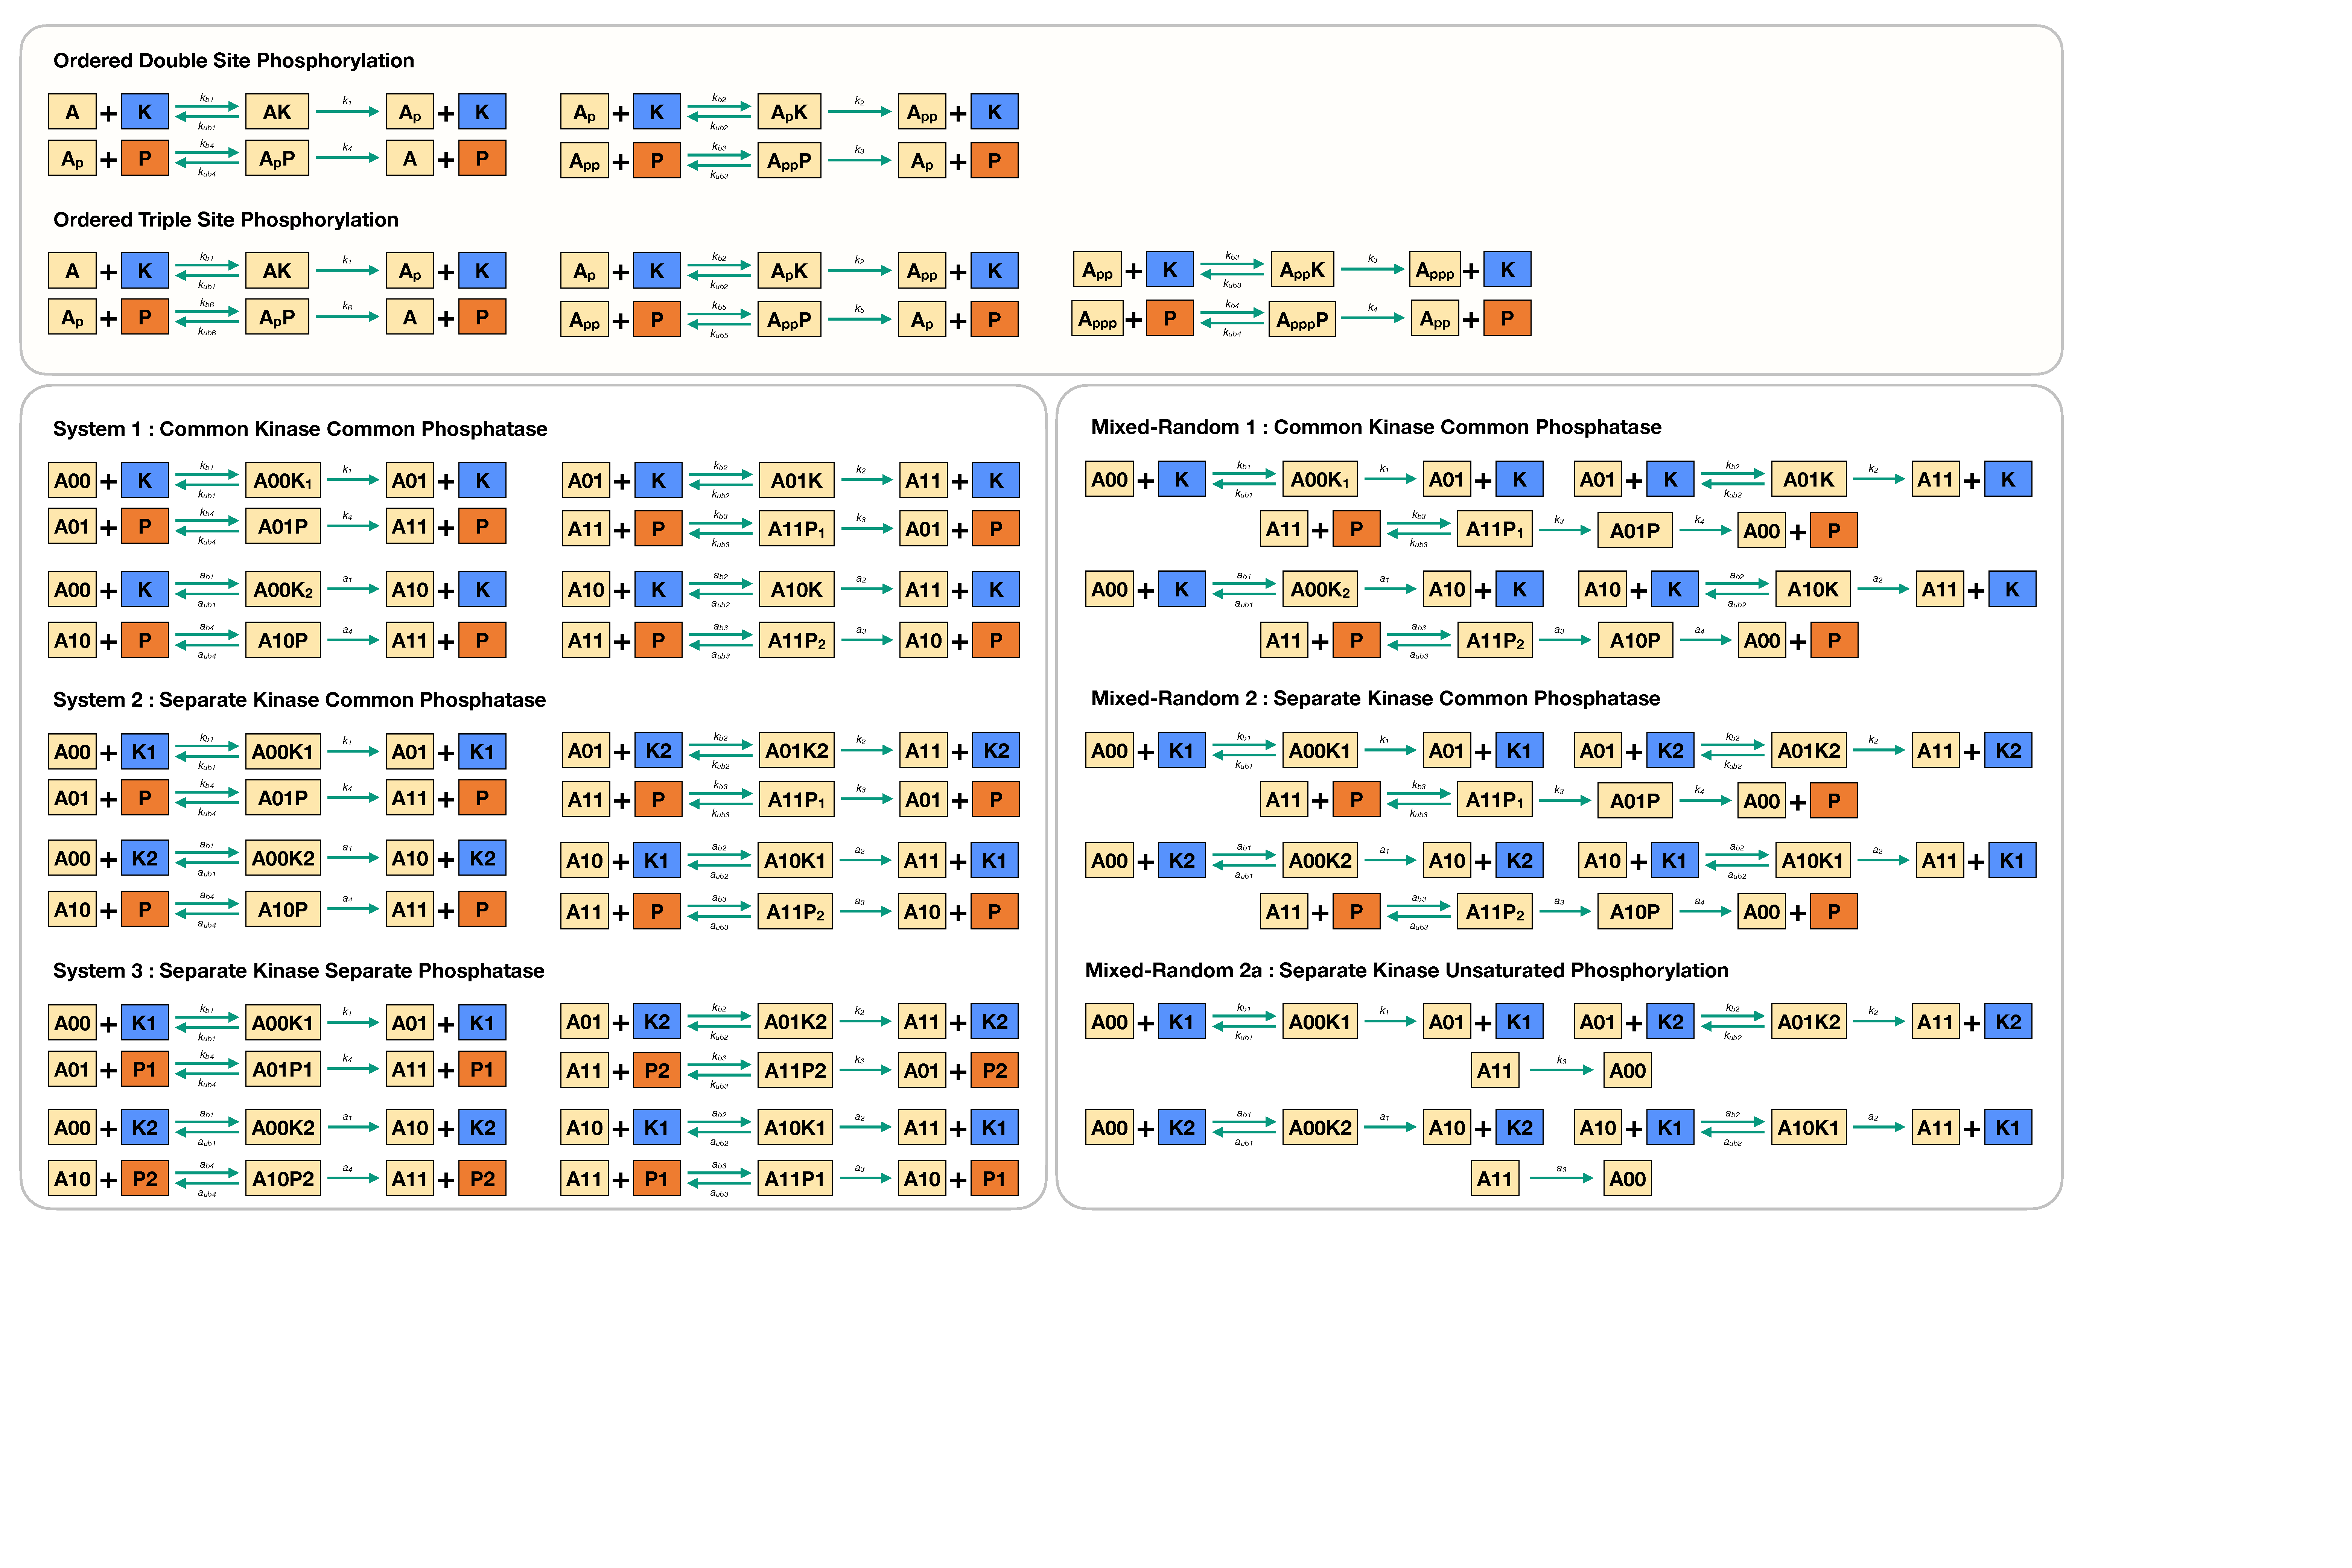
\includegraphics[width = 0.9\paperwidth,  keepaspectratio]{Supplementary_Figures/FigS10.pdf}
    \caption{\textbf{Detailed model description of the various MSP networks used in this paper.} The constituent binding, unbinding and catalytic reactions of each modification step is described in detail and are modelled using mass kinetic description.}
    \label{Fig S10}
\end{figure}


\end{document}
